\documentclass[nochapter]{tcd-msc-hpc}
\thesis{MSc in High-performance Computing}
\school{School of Mathematics}

%Fill in this information with details about yourself and your project
\title{Communication-Avoiding Krylov Subspace Methods for Option Pricing}
\shorttitle{CAKSM for Option Pricing}
\author{Kevin Knights}
\studentID{25378095}
\firstsupervisor{Kirk M. Soodhalter}
%\secondsupervisor{}
\submissiondate{Date your submitted your thesis}
\signaturefile{sig.png}%file containing your signature for plagiarism pledge
\signaturewidth{0.3}%as a percentage between 0 and 1 to adjust signature size
\codelink{https://github.com/kevinknights29/caksm}

% Imports
\usepackage{amsmath,amssymb,amsfonts}
\usepackage{mathtools}
\usepackage{bm}
\usepackage{booktabs}
\usepackage{lastpage}
\newcommand{\R}{\mathbb{R}}
\newcommand{\vect}[1]{\mathbf{#1}}
\newcommand{\mat}[1]{\mathbf{#1}}
\newcommand{\Rv}{R_v}
\newcommand{\Rh}{R_h}

\begin{document}
\maketitle

\newpage

\makeplagiarismpage

\newpage

\section*{Acknowledgements}
Write acknowledgements to your supervisor, classmates, friends, family, partner\ldots anyone who supported you during the MSc.

\newpage
\begin{abstract}
\section*{Abstract}
A trading desk repricing a multi-asset option book revalues the same partial differential
equation thousands of times a day, and at production resolution a single price costs on the
order of hundreds of seconds. The bottleneck is not arithmetic: a Krylov exponential
integrator spends over 70\% of its time in sparse matrix--vector products that move far more
bytes than they compute, and most of the rest in an orthogonalization whose every step is a
global synchronization. Communication-avoiding (CA) reformulations attack exactly these two
costs, but whether the trade pays depends on the operator, the grid, and the machine.

This thesis answers \emph{when} it pays, in coordinates that transfer. A benchmark pricer
implementing five methods on two 3-asset European options establishes an uncompromised
baseline and reproduces the reference results of Niesen and Wright. A regime study then
builds a dimensionless map of the CA design space: a vertical axis $\Rv$ (working set over
aggregate last-level cache) governing matrix-powers tiling, and a horizontal axis $\Rh$
(reduction cost over compute between reductions) governing $s$-step orthogonalization, with
predicted crossovers at 1. The map's coordinates are predictors computed before any run;
measurements test the boundaries and never enter a coordinate. The certified $s$-step block
width is predicted from the spectrum alone and verified integer-exact on 20 of 21 runs; a
log-robustness law bounds the damage non-normality does to that prediction; and a
closed-form tensor law gives the growth of eigenvector conditioning with asset dimension.
On the measurement side the study delivers one null result with a mechanism (the horizontal
reduction cut does not move wall-clock, exactly as the map predicts), one shortfall with a
mechanism (cache-blocked matrix powers trades halo arithmetic for DRAM traffic at a loss),
and a placed trajectory showing the production operator to be squarely in vertical-only
territory. A planned GPU study, outlined here, will test the map's central portability
claim on a memory system that differs in kind.
\\
\newline
\textbf{Keywords:} Krylov subspace methods, communication-avoiding algorithms, matrix
exponential, option pricing, roofline model, $s$-step methods, performance modeling
\end{abstract}
\vspace{8pt}
\tableofcontents
\newpage
\addcontentsline{toc}{section}{Lists of Figures and Tables}
\listoffigures
\listoftables
\newpage
%%%%%%%%%%%%%%%%%%%%%%%%%%%%%%%%%%%%%%%%%%%%%%%%%%%%%%%%%%%%%%%%%%%%%%%%%%%%%%%%%%%
\setcounter{section}{0}
\section{Introduction}\label{sec:intro}

A trading desk repricing a multi-asset book revalues the same PDE thousands of times a day,
so the wall-clock cost of one solve sets what can be quoted, hedged, and risk-managed
intraday. For a 3-asset basket at a resolution fine enough to matter, the published cost is
roughly 700\,s per price \cite{niesen-wright-2012}. The bottleneck is not arithmetic. A
Krylov exponential integrator spends over 70\% of its time in sparse matrix--vector products
(SpMV) that move far more bytes than they compute, and the rest in an orthogonalization
whose every step is a global synchronization. Both are \emph{communication} costs: data
crossing the memory hierarchy, and cores waiting on each other
\cite{ballard-2011,hoemmen-2010}. Communication-avoiding (CA) reformulations attack exactly
these---matrix powers computes $s$ Krylov vectors per pass over the operator instead of one
\cite{demmel-2008,mohiyuddin-2009}, and $s$-step orthogonalization replaces $O(m^2)$
reductions with $O(m/s)$ \cite{hoemmen-2010,carson-2015}---trading redundant arithmetic,
which is cheap, for movement and latency, which are not.

Whether that trade pays is not a property of the algorithm. It depends on the operator, the
grid, and the machine. This thesis answers \emph{when} it pays, and does so in coordinates
that transfer.

Two artifacts support that answer. A \textbf{benchmark pricer} in C++23 implements five
methods (Crank--Nicolson, two ADI variants, a one-shot matrix exponential, and a Krylov
exponential integrator) on two 3-asset European options, and establishes the uncompromised
baseline the CA work must beat (\Cref{sec:benchmark}). A \textbf{regime study}
(\Cref{sec:regime}) builds a dimensionless map of the CA design space: because both of its
axes are ratios rather than absolute times, the map is independent of the machine and of
the problem, so a reader can place their own operator and hardware on it and read off which
mechanism, if either, can pay for them. The CA Krylov exponential integrator itself is not
yet implemented; the map exists to decide what to build.

The design rule that keeps the map non-circular is stated up front because everything else
depends on it: \emph{coordinates are predictors}, computed before a run from the problem
size, the sparsity pattern, the spectrum, and the machine constants; \emph{outcomes}
(wall-clock, orthogonality loss, achieved bytes) test the boundaries and never enter a
coordinate.

The thesis proceeds as follows. \Cref{sec:model} states the pricing problem and its
discretization. \Cref{sec:ksm} presents the Krylov exponential integrator, its cost
structure, and the CA reformulations that target it. \Cref{sec:platform} describes the
experimental platform and measurement methodology. \Cref{sec:benchmark} reproduces the
Niesen--Wright benchmark as a control. \Cref{sec:profile} profiles the solver and places
its kernels on a cache-aware roofline. \Cref{sec:scaling} presents the OpenMP scaling study
that motivates the two CA mechanisms. \Cref{sec:regime} develops the regime map and its
numerical and measured results. \Cref{sec:gpu} outlines the GPU study now in progress,
which is designed as a falsification test of the map's central claim. \Cref{sec:conclusion}
concludes.

%%%%%%%%%%%%%%%%%%%%%%%%%%%%%%%%%%%%%%%%%%%%%%%%%%%%%%%%%%%%%%%%%%%%%%%%%%%%%%%%%%%
\section{The pricing problem and its discretization}\label{sec:model}

The model problem is the 3-asset Black--Scholes PDE \cite{black-scholes-1973} in log-price
coordinates, solved backward in pseudo-time $\tau$ from 0 (payoff) to $T$ (price):
\begin{equation}
\frac{\partial u}{\partial \tau}
= \frac{1}{2} \sum_{d,d'} \rho_{dd'} \sigma_d \sigma_{d'}
  \frac{\partial^2 u}{\partial x_d \partial x_{d'}}
+ \sum_d \left(r - \tfrac{1}{2}\sigma_d^2\right) \frac{\partial u}{\partial x_d}
- r\, u + b(\tau).
\label{eq:bs-pde}
\end{equation}
Two payoffs are priced. The basket call,
\[
u_0(x) = \max\!\Big(\sum_d w_d e^{x_d} - K,\ 0\Big),
\]
and the rainbow min-call,
\[
u_0(x) = \max\!\Big(\min_d e^{x_d} - K,\ 0\Big).
\]
The boundary forcing term $b(\tau)$ for the basket case is encoded as a polynomial
$B \cdot s(\tau)$ with $s(\tau) = [\tau^2/2,\ \tau,\ 1]^\top$, derived from a deep
in-the-money approximation on ghost nodes outside the grid. The rainbow case uses modified
finite-difference stencils (a zero-gamma boundary condition) instead.

Discretization is by second-order central differences on a uniform Cartesian grid with
$x_1$-fastest lexicographic ordering, so every operator is a three-fold Kronecker product
with identity in the undifferentiated directions. The assembled $\mat{A}$ carries at most
19 nonzeros per row (a 7-point stencil plus $3 \times 4$ mixed-derivative diagonals). Its
bandwidth is $O(N_1 N_2)$, set by the $x_3$ and mixed terms, which rules out banded direct
solvers at scale. $\mat{A}$ splits as $\mat{A}_{\text{sym}} + \mat{A}_{\text{skew}}$---%
diffusion, mixed, and reaction terms symmetric, convection skew-symmetric---so it is not
symmetric in general, but $\operatorname{Re}(\lambda) \le 0$ holds, which is what stability
of $e^{h\mat{A}}$ requires. \Cref{tab:params} lists the default model parameters used
throughout.

\begin{table}[htbp]
\centering
\caption{Default model parameters.}
\label{tab:params}
\begin{tabular}{@{}lll@{}}
\toprule
\textbf{Parameter} & \textbf{Value} & \textbf{Description} \\
\midrule
Spot prices $S_0$        & $(100, 100, 100)$    & Initial asset prices \\
Strike $K$               & 100                  & Option strike \\
Risk-free rate $r$       & 0.04                 & Continuously compounded \\
Maturity $T$             & 1.0 year             & Fixed \\
Volatilities $\sigma$    & $(0.30, 0.35, 0.40)$ & Per-asset annual volatility \\
Correlations $\rho$      & $(0.50, 0.50, 0.50)$ & Off-diagonal pairs $(\rho_{01}, \rho_{02}, \rho_{12})$ \\
Basket weights $w$       & $(1/3, 1/3, 1/3)$    & Equal-weight basket \\
Grid half-width $\alpha$ & 2.85                 & Domain $\pm \alpha \sigma \sqrt{T}$ per dimension \\
\bottomrule
\end{tabular}
\end{table}

Stiffness grows sharply with refinement: the smallest eigenvalue moves from $-24$ at grid
size $n=11$ to $-2924$ at $n=101$ (where $N = n^3$ is the total number of unknowns).
Over-solving in time on a coarse grid is therefore pointless, and the commercial motivation
sits at the other end: Niesen and Wright report ${\sim}700$\,s for Hundsdorfer--Verwer to
reach one basis point at $61^3$ \cite{niesen-wright-2012}.

%%%%%%%%%%%%%%%%%%%%%%%%%%%%%%%%%%%%%%%%%%%%%%%%%%%%%%%%%%%%%%%%%%%%%%%%%%%%%%%%%%%
\section{The Krylov exponential integrator}\label{sec:ksm}

After spatial discretization, the semi-discrete system takes the affine form
\begin{equation}
  \frac{d\vect{u}}{d\tau} = \mat{A}\vect{u} + \vect{b}, \qquad \vect{u}(\tau_0) = \vect{u}_0.
  \label{eq:ode}
\end{equation}
Following Niesen and Wright \cite{niesen-wright-2012}, the inhomogeneity is absorbed into an
\emph{extended system}: define
\[
  \widetilde{\mat{A}} =
  \begin{bmatrix} \mat{A} & \vect{b} \\ \vect{0}^T & 0 \end{bmatrix}
  \in \R^{(N+1)\times(N+1)},
  \qquad
  \widetilde{\vect{v}} =
  \begin{bmatrix} \vect{u}_k \\ 1 \end{bmatrix}
  \in \R^{N+1},
\]
so that the exact solution at time $\tau_0 + h$ is encoded in the first $N$ components of
$e^{h\widetilde{\mat{A}}}\widetilde{\vect{v}}$.

The Krylov approximation proceeds via the Arnoldi iteration on $\widetilde{\mat{A}}$ with
starting vector $\widetilde{\vect{v}}$, producing an orthonormal basis $\mat{V}_m$ and an
upper Hessenberg matrix $\overline{\mat{H}}_m \in \R^{(m+1)\times m}$
\cite{saad-1992,hochbruck-lubich-1997}. Dropping the last row gives
$\mat{H}_m \in \R^{m\times m}$, and the approximation reads
\begin{equation}
  e^{h\widetilde{\mat{A}}}\widetilde{\vect{v}}
  \;\approx\;
  \beta\, \mat{V}_m\, e^{h \mat{H}_m} \vect{e}_1,
  \qquad
  \beta = \|\widetilde{\vect{v}}\|.
  \label{eq:krylov_approx}
\end{equation}
Algorithm~\ref{alg:krylov_exp} gives the full adaptive procedure, and
Algorithm~\ref{alg:arnoldi} the Arnoldi iteration it calls.

\begin{algorithm}[htbp]
\caption{Adaptive Krylov Exponential Integrator for
$\vect{u}' = \mat{A}\vect{u} + \vect{b}$}
\label{alg:krylov_exp}
\KwIn{Matrix $\mat{A} \in \R^{N \times N}$, vector
      $\vect{b} \in \R^N$, initial condition $\vect{u}_0$,
      final time $T$, time-step $\Delta\tau$,
      tolerance $\texttt{tol}$}
\KwOut{Solution snapshots $\{\vect{u}_k\}_{k=0}^{K}$ at
       $\tau_k = k\,\Delta\tau$}
$\tau \gets 0$\;
\For{$k = 0, 1, \ldots, K-1$}{
  $h \gets \min(\Delta\tau,\; T - \tau)$\;
  $m \gets 1$;\quad $\texttt{err} \gets \infty$\;
  \BlankLine
  \tcc{Form extended system}
  $\widetilde{\mat{A}} \gets
     \begin{bmatrix} \mat{A} & \vect{b} \\[2pt]
     \vect{0}^T & 0 \end{bmatrix}
     \in \R^{(N+1)\times(N+1)}$\;
  $\widetilde{\vect{v}} \gets
     \begin{bmatrix} \vect{u}_k \\ 1 \end{bmatrix}
     \in \R^{N+1}$\;
  \BlankLine
  \tcc{Adaptive Krylov loop}
  \While{$m \le N+1$}{
    Run $m$ steps of Arnoldi on
        $(\widetilde{\mat{A}},\,\widetilde{\vect{v}})$
        $\;\Rightarrow\;$
        $\mat{V}_{m+1},\; \overline{\mat{H}}_m$
        \tcp{Algorithm~\ref{alg:arnoldi}}
    Store $\bar{h}_{m+1,m} \gets [\overline{\mat{H}}_m]_{m+1,m}$
        \tcp{sub-diagonal entry}
    $\mat{H}_m \gets \overline{\mat{H}}_m(1{:}m,\;1{:}m)$
        \tcp{drop last row}
    $\beta \gets \|\widetilde{\vect{v}}\|$\;
    $\vect{f} \gets e^{h\,\mat{H}_m}\,\vect{e}_1$
        \tcp{small $m\times m$ matrix exponential}
    $\vect{w} \gets \beta\;\mat{V}_m\;\vect{f}$
        \tcp{Krylov approximation in full space}
    \BlankLine
    \tcc{A posteriori error estimate}
    $\texttt{err} \gets |\bar{h}_{m+1,m}|\;\cdot\;|[\vect{f}]_m|$\;
    \If{$\texttt{err} < \texttt{tol}$}{
      \textbf{break}\;
    }
    $m \gets m + 1$\;
  }
  $\vect{u}_{k+1} \gets \vect{w}(1{:}N)$
      \tcp{extract first $N$ components}
  $\tau \gets \tau + h$\;
}
\end{algorithm}

\begin{algorithm}[htbp]
\caption{Arnoldi Iteration}
\label{alg:arnoldi}
\KwIn{Matrix $\widetilde{\mat{A}} \in \R^{(N+1) \times (N+1)}$,
      vector $\widetilde{\vect{v}} \in \R^{N+1}$,
      subspace dimension $m$,
      breakdown tolerance $\texttt{tol}$}
\KwOut{Orthonormal basis $\mat{V}_{m+1} \in \R^{(N+1)\times(m+1)}$,
       upper Hessenberg $\overline{\mat{H}}_m \in \R^{(m+1)\times m}$}
$\beta \gets \|\widetilde{\vect{v}}\|$;\quad
$\vect{v}_1 \gets \widetilde{\vect{v}} / \beta$\;
\For{$j = 1, \ldots, m$}{
  $\vect{w} \gets \widetilde{\mat{A}}\,\vect{v}_j$\;
  \For{$i = 1, \ldots, j$}{
    \tcp{Modified Gram--Schmidt}
    $h_{i,j} \gets \vect{v}_i^T \vect{w}$\;
    $\vect{w} \gets \vect{w} - h_{i,j}\,\vect{v}_i$\;
  }
  $h_{j+1,j} \gets \|\vect{w}\|$\;
  \If{$h_{j+1,j} < \texttt{tol}$}{
    \textbf{break} \tcp{Invariant subspace found (happy breakdown)}
  }
  $\vect{v}_{j+1} \gets \vect{w} / h_{j+1,j}$\;
}
\end{algorithm}

\subsection{Cost structure and the sequential dependency}\label{sec:ksm-cost}

The dominant cost of the integrator is the Arnoldi iteration. Each step $j$ requires one
sparse matrix--vector product $\vect{w} = \widetilde{\mat{A}}\vect{v}_j$, costing $O(N)$,
and orthogonalization against all previous vectors, costing $O(jN)$. Crucially, step $j$
cannot begin until $\vect{v}_j$ is available, which requires step $j-1$ to have completed.
This creates a strictly sequential data dependency across the Krylov dimension $m$. The
individual SpMV and inner products within each step can be parallelized, but this inner
parallelism scales poorly: the SpMV is bandwidth-bound, and every inner product in the
modified Gram--Schmidt (MGS) loop is a global reduction. These are the two
\emph{communication} walls, and they are different in kind:

\begin{table}[htbp]
\centering
\caption{The two kernels, their bounds, and the CA mechanism each motivates.}
\label{tab:two-mechanisms}
\begin{tabular}{@{}lllp{4.3cm}@{}}
\toprule
\textbf{Kernel} & \textbf{Bound} & \textbf{Communication} & \textbf{CA mechanism} \\
\midrule
SpMV         & bandwidth (memory hierarchy)    & vertical   & matrix powers / cache blocking \\
Gram--Schmidt & synchronization (reductions)   & horizontal & $s$-step / block orthogonalization \\
\bottomrule
\end{tabular}
\end{table}

\subsection{Communication-avoiding reformulations}\label{sec:ksm-ca}

The $s$-step (CA-Arnoldi) reformulation \cite{hoemmen-2010,demmel-2008,carson-2015}
computes $s$ basis vectors $\vect{v}, \mat{A}\vect{v}, \ldots, \mat{A}^s\vect{v}$ per
communication phase. The \emph{matrix-powers kernel} \cite{mohiyuddin-2009} computes all
$s$ products in one pass over the operator, tiling the grid so that each panel and its
$s$-deep halo stay cache-resident---attacking the vertical wall. The block is then
orthogonalized at once---here by CholeskyQR2 \cite{yamamoto-2015}, whose certificate
$\kappa(\mat{B}) \le u^{-1/2}$ (with $u$ the unit roundoff) is a floating-point theorem
rather than a machine property---attacking the horizontal wall with $O(m/s)$ reductions in
place of MGS's $O(m^2)$. The cost is conditioning: the monomial basis
$[\vect{v}, \mat{A}\vect{v}, \ldots, \mat{A}^s\vect{v}]$ grows geometrically
ill-conditioned in $s$, which caps the usable block width. Quantifying that cap---%
predicting it from the spectrum, certifying it, and measuring where the prediction
survives non-normality---is a central thread of \Cref{sec:regime}.

An alternative not pursued here is the rational Krylov subspace
\cite{berljafa-guttel-2017}, which replaces the sequential polynomial recurrence with $m$
independent shifted solves. Its parallelism is attractive, but each solve is itself a
sparse linear system whose iterative solution re-imports both communication walls, and the
near-optimal pole selection adds problem-specific tuning. The $s$-step route was chosen
because its costs are analyzable in machine terms---which is precisely what the regime map
requires.

%%%%%%%%%%%%%%%%%%%%%%%%%%%%%%%%%%%%%%%%%%%%%%%%%%%%%%%%%%%%%%%%%%%%%%%%%%%%%%%%%%%
\section{Experimental platform and methodology}\label{sec:platform}

Every result in this thesis was gathered on a single bare-metal workstation
(``puffin''): an AMD Ryzen Threadripper 3960X, 24 cores in a single socket and a single
NUMA node, organized as 8 core complexes (CCX) of 3 cores, each CCX with its own 16\,MiB
slice of L3 (128\,MiB total). Per-core caches are 32\,KiB L1d and 512\,KiB L2; nominal
maximum clock is 3.8\,GHz, and main memory is 4-channel DDR4-3200 with a theoretical
102.4\,GB/s roof. The machine also hosts an NVIDIA RTX~3090 (24\,GB), which plays a role
in the GPU outlook of \Cref{sec:gpu}. The machine's derived constants live in a single
header (\texttt{include/machine.hpp}) under the key \texttt{amd-3960x}, and every predicted
coordinate in the regime study is computed from them.

\paragraph{Why one bare-metal machine, and not a cloud VM.} An earlier cloud arm was
dropped, on two grounds. Contention: timing variance that looks internally consistent is
simultaneously evidence of memory-bound behavior and of noise from co-tenants, and from
inside the guest the two are not separable. Topology, the sharper objection: the hypervisor
reports a socket and a private last-level cache slice \emph{per vCPU}---a fiction of the
virtualization rather than the silicon. Both coordinates of the regime map are functions of
real cache geometry (one is a cache-capacity ratio, the other is set by how many
cache-domain boundaries a reduction tree crosses), so neither is knowable on an invented
topology, and the map cannot be drawn there at all. Bare metal removes the hypervisor but
not OS scheduling noise, so every timed quantity below is reported as a median with an
inter-quartile range over repeated trials; on a boost-enabled chip timing noise is
right-skewed, and the median reports a \emph{sustainable} throughput where the minimum
would report an unsustainable boost spike.

\paragraph{Vectorization is not the baseline's problem.} A STREAM Triad
\cite{mccalpin-1995} sweep built with default flags (SSE2) and with
\texttt{-march=native} (AVX2) is identical inside run-to-run spread---22.8 vs.\
22.6\,GB/s at one thread, 39.3 vs.\ 39.5\,GB/s at the 24-thread saturation knee, against
the 102.4\,GB/s theoretical roof (\Cref{fig:stream}). On a bandwidth-bound kernel the
instruction set buys nothing, so the CPU baseline is fair as measured.

\begin{figure}[htbp]
\centering
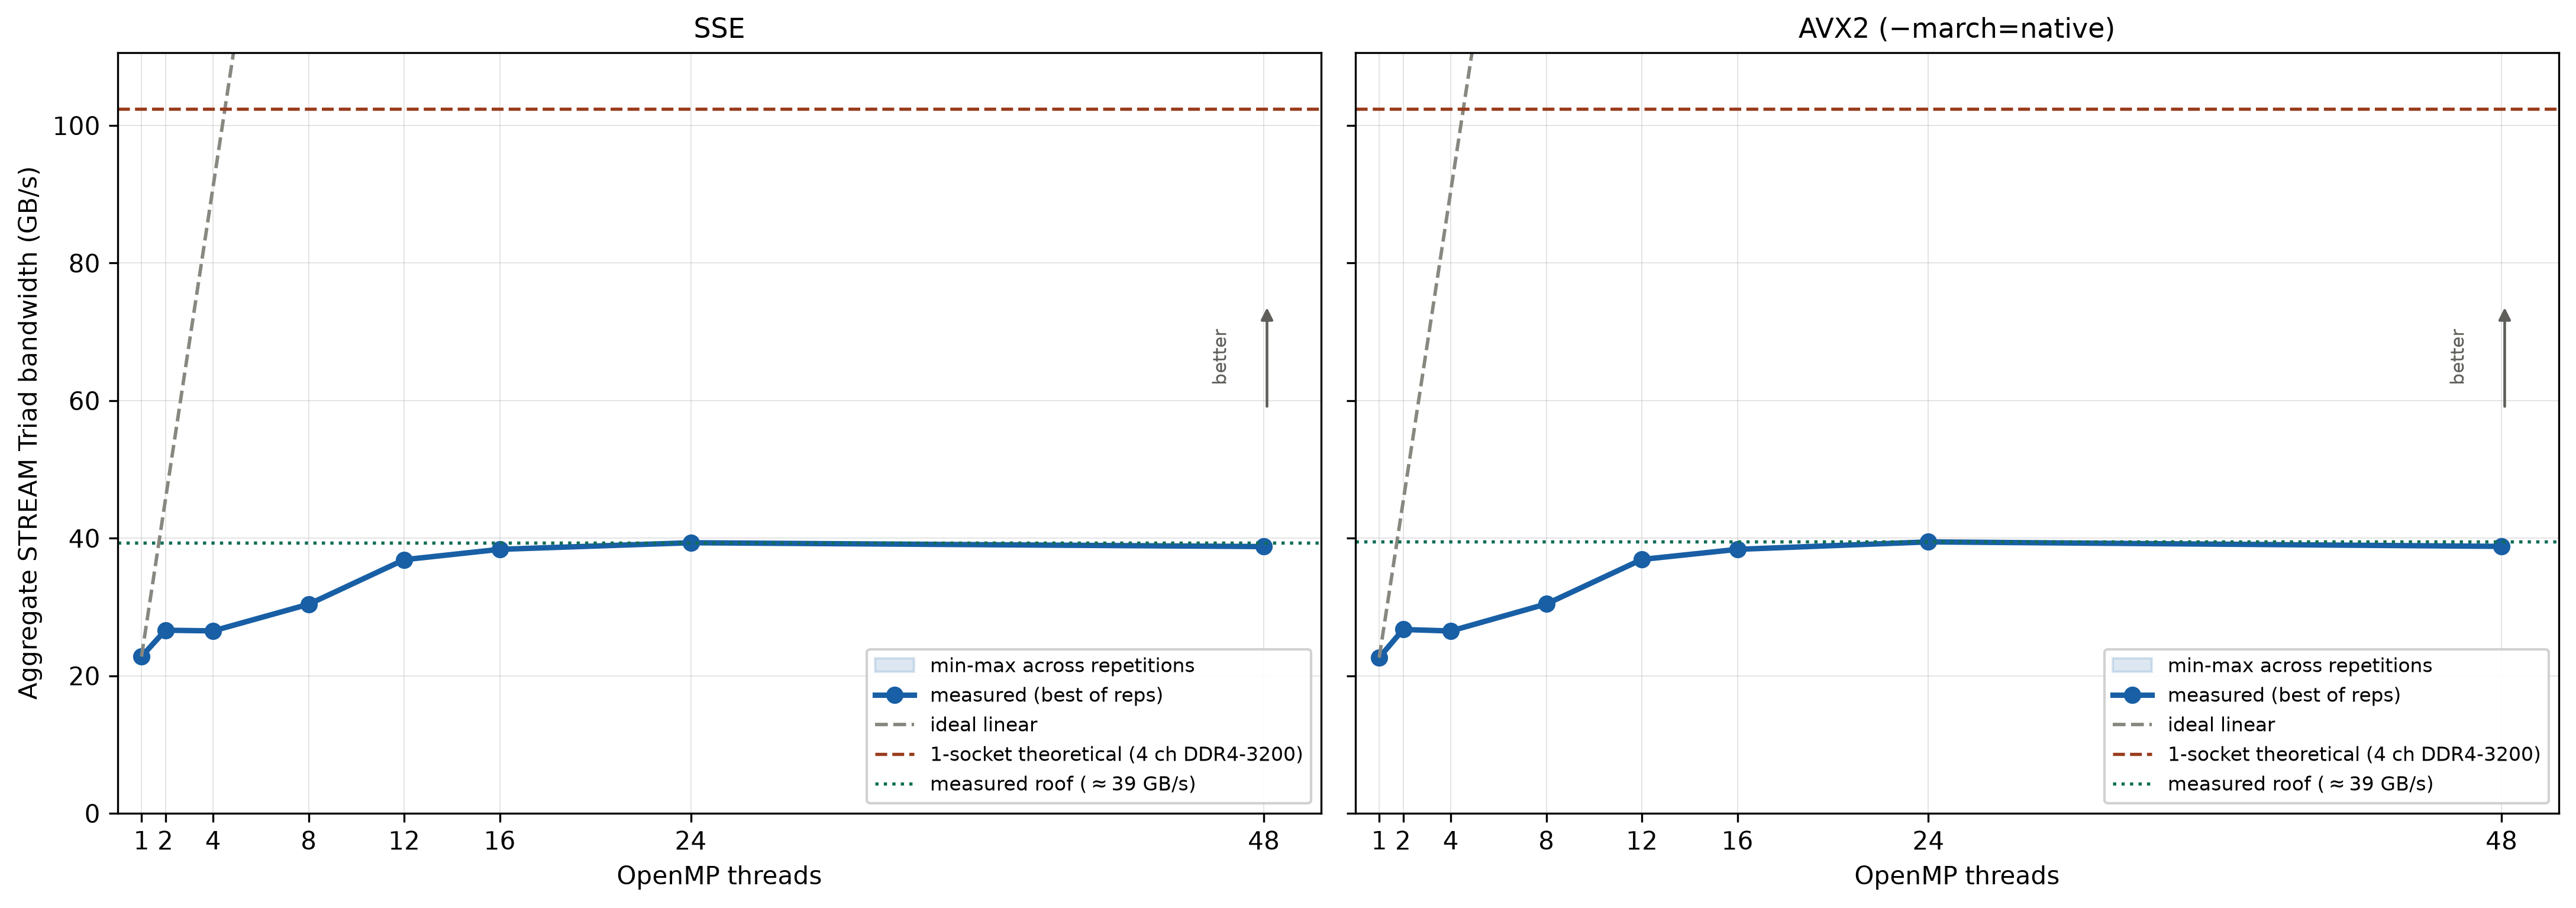
\includegraphics[width=0.9\textwidth]{stream_sweep.png}
\caption{STREAM Triad bandwidth sweep, SSE2 vs.\ AVX2 builds. The two instruction sets are
indistinguishable at every thread count: the kernel is bandwidth-bound, not
vectorization-bound.}
\label{fig:stream}
\end{figure}

\paragraph{Reproducibility.} Every number quoted in this thesis names the script that
reproduces it. The repository builds with CMake and GCC~16 (C++23); sweep scripts write
CSVs under \texttt{data/}, which is generated locally and excluded from version control
precisely so that no quoted figure can drift from its generating run; each figure is
produced by a self-contained plotting script with inline dependency metadata. The regime
executables read machine constants from a single audited header, so porting the study to a
new machine is a matter of deriving one new constants block---a property the GPU study of
\Cref{sec:gpu} depends on.

%%%%%%%%%%%%%%%%%%%%%%%%%%%%%%%%%%%%%%%%%%%%%%%%%%%%%%%%%%%%%%%%%%%%%%%%%%%%%%%%%%%
\section{Benchmark: reproducing Niesen--Wright}\label{sec:benchmark}

Five methods are compared. Three are time-steppers over a fixed number of substeps:
Crank--Nicolson ($\theta = 0.5$, fully implicit, second order, one sparse LU factorization
per run), and two alternating-direction-implicit splittings---Douglas--Rachford
\cite{douglas-rachford-1956}, with three direction-split solves per step, and
Hundsdorfer--Verwer \cite{hundsdorfer-verwer-2003,inthout-foulon-2010}, a
Douglas--Rachford predictor with a corrector. The remaining two exponentiate the operator: \textsf{ME} forms
$e^{T\widetilde{\mat{A}}}$ in one shot by scaling and squaring
\cite{higham-2005,almohy-higham-2011} with an $\infty$-norm early exit, choosing its own
substep count; \textsf{KSM-EI} is the Krylov exponential integrator of \Cref{sec:ksm},
growing the basis until an a-posteriori estimate meets the tolerance.

The benchmark reproduces Figure~1 of Niesen and Wright \cite{niesen-wright-2012}: log-log
plots of ODE error against CPU time for all five methods, across both option types and both
grid sizes (\Cref{fig:benchmark}).

\begin{figure}[htbp]
\centering
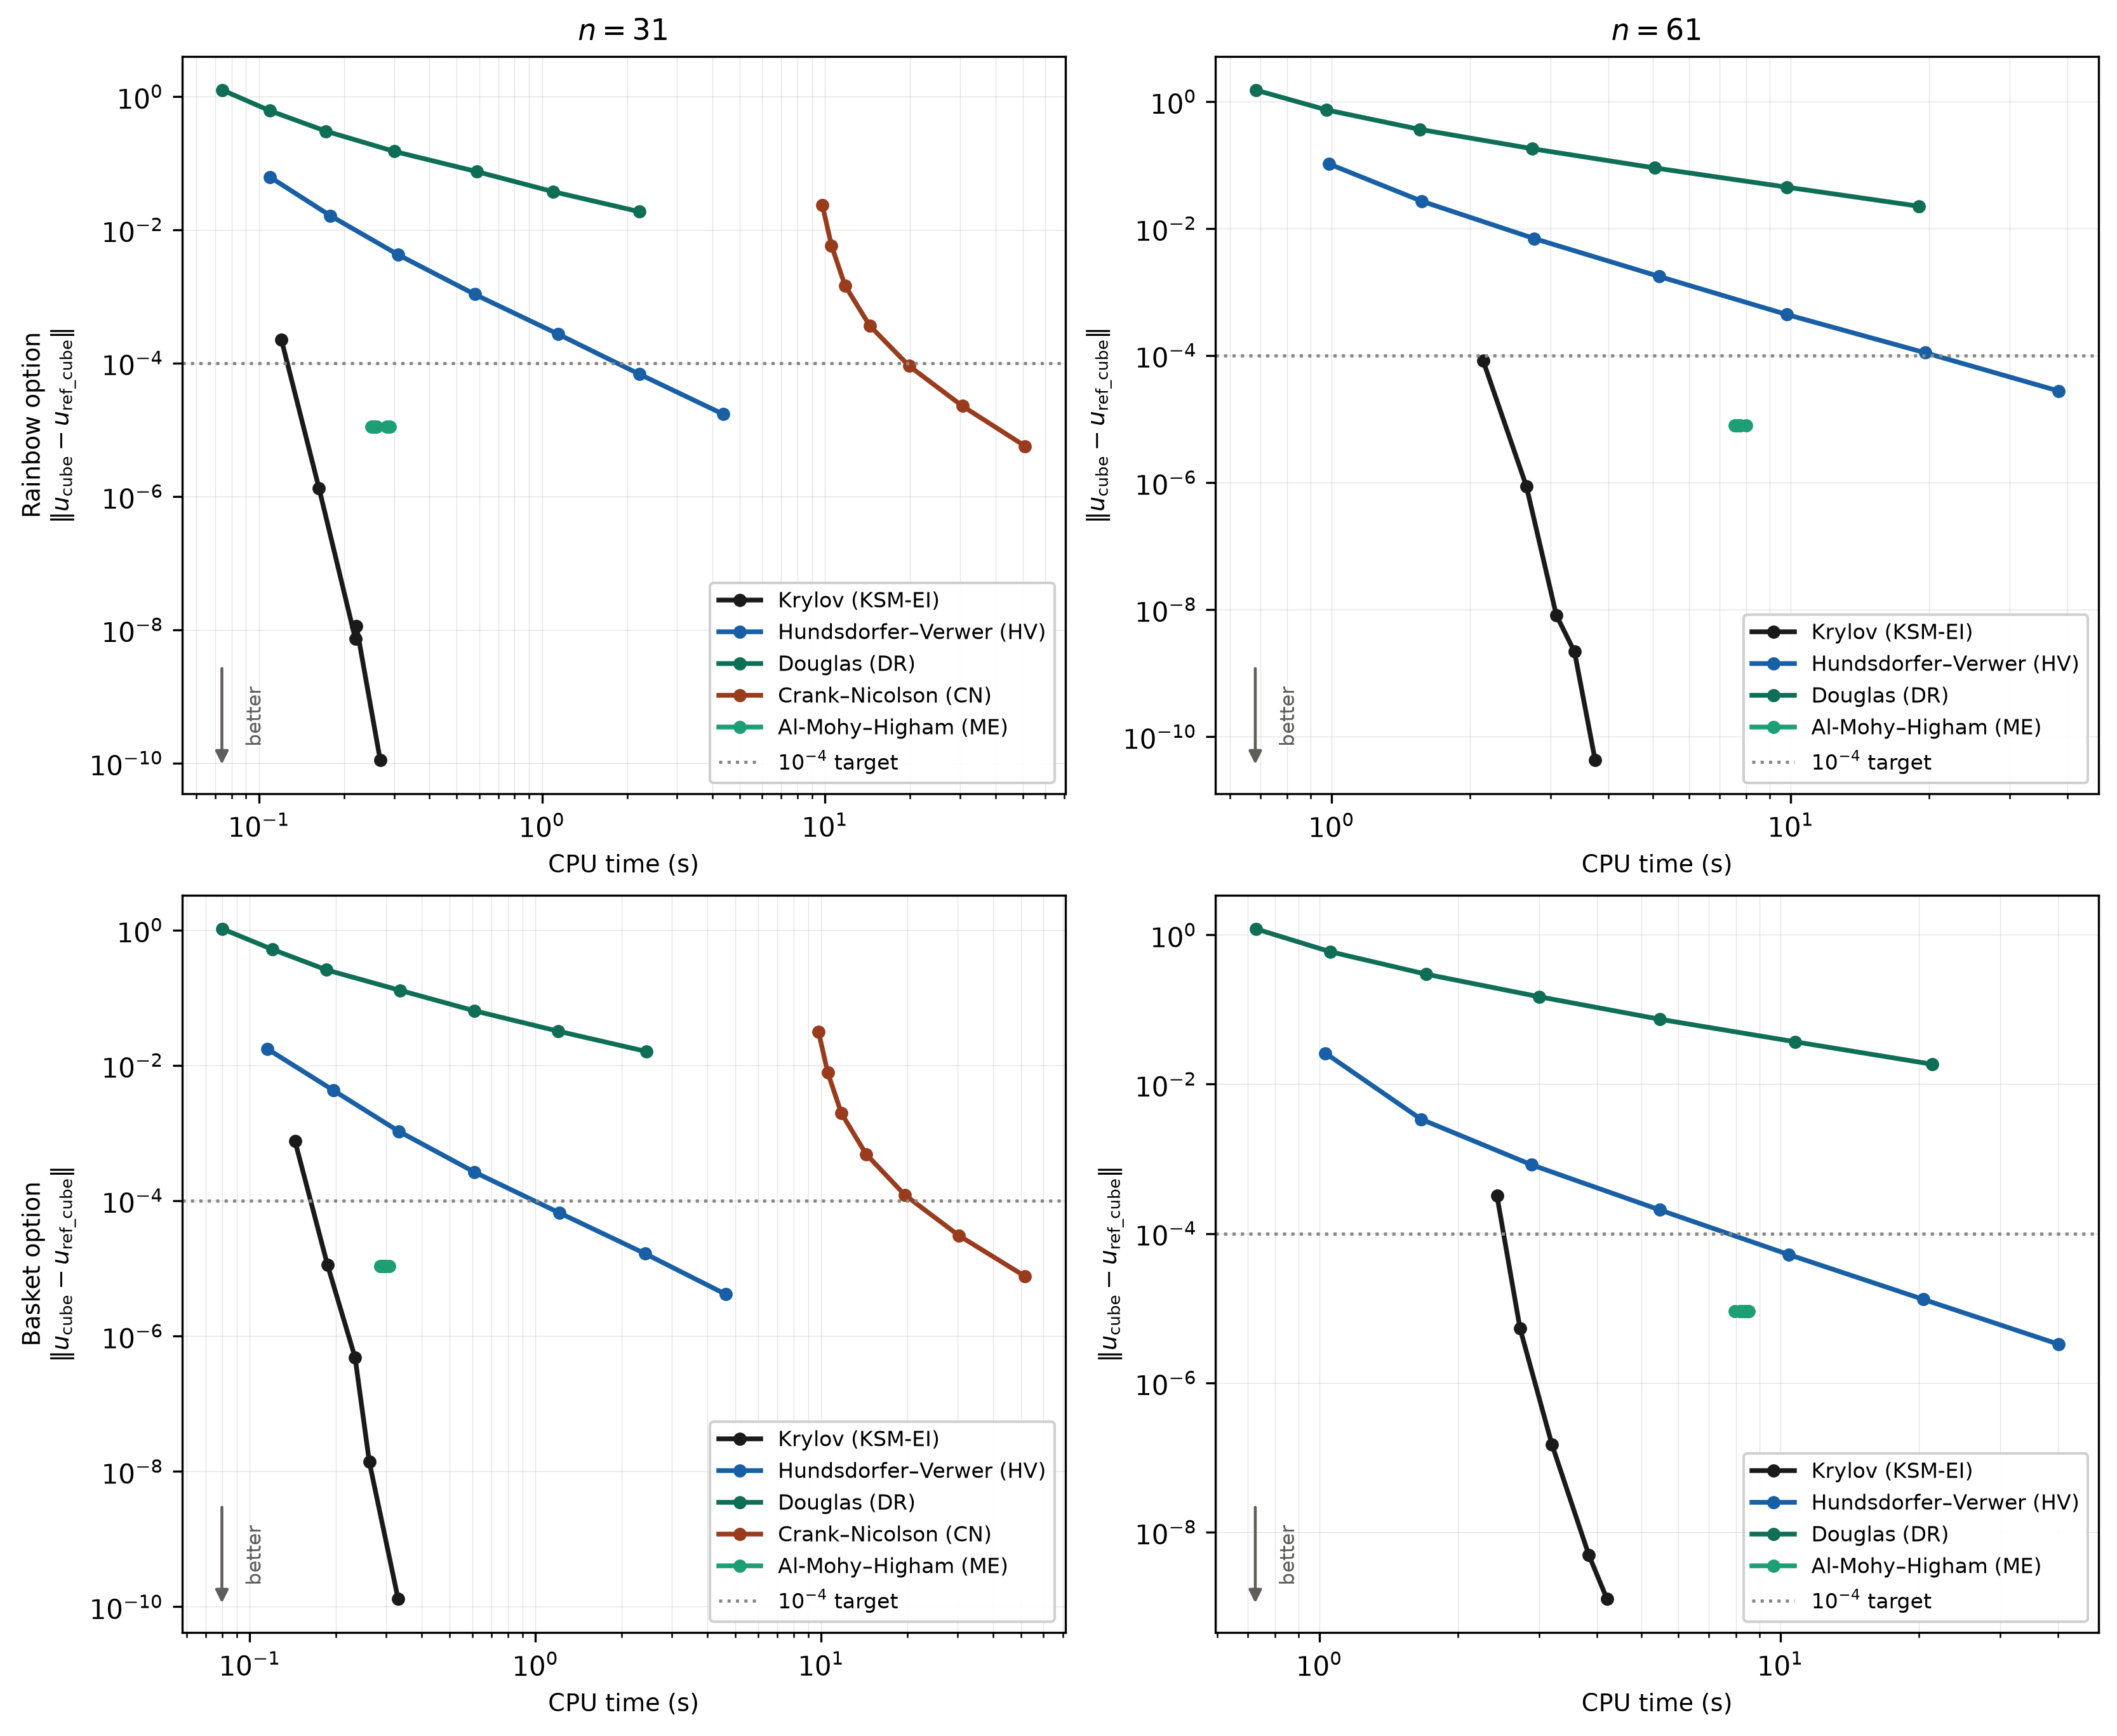
\includegraphics[width=\textwidth]{benchmark_plots.png}
\caption{ODE error vs.\ CPU time for the five methods, across both payoffs and grid sizes,
reproducing Niesen--Wright Figure~1. The Krylov integrator dominates in the
${\sim}10^{-4}$ accuracy band; Crank--Nicolson's non-monotone stiff-mode ringing
($R(-\infty) = -1$) is visible as predicted.}
\label{fig:benchmark}
\end{figure}

\paragraph{The referee.} The measurement is against the exact ODE solution, not the
analytic price. Before each option type is benchmarked, a high-accuracy matrix-exponential
referee is computed at maximum Taylor degree $m = 55$ and $\theta = 9.9$, giving
$s = \lceil T \lVert \widetilde{\mat{A}} \rVert_1 / \theta \rceil$ internal substeps at a
tolerance of $2^{-53} \approx 1.1 \times 10^{-16}$. Scoring against the analytic price
instead would fold spatial discretization error into a claim about time integration, so the
referee is deliberately a different object from the contestants: the exact solution of the
same semi-discrete system. The error is the Euclidean norm over the $9 \times 9 \times 9$
grid neighborhood centered on the spot rather than the value at a single node, so a lucky
cancellation at one grid point cannot flatter a method.

\paragraph{Control, not result.} The method ordering matches theory, and that is the point
of this section: it is the \emph{control} for everything after it. On an autonomous linear
problem the one-shot matrix exponential is genuinely hard to beat: at $n=15$ time-exactness
buys nothing, because every method is already pinned at the spatial error (0.066). The
Krylov integrator's structural advantages---adaptivity, no step-count trial-and-error, and
a retained trajectory that a one-shot exponential discards---only cash out away from this
benign regime, at the production resolutions where the ${\sim}700$\,s cost lives.

%%%%%%%%%%%%%%%%%%%%%%%%%%%%%%%%%%%%%%%%%%%%%%%%%%%%%%%%%%%%%%%%%%%%%%%%%%%%%%%%%%%
\section{Profile and roofline}\label{sec:profile}

At $n=61$ (226{,}981 unknowns, 4.23M nonzeros, ${\approx}49$\,MB in compressed sparse
column form) over 100 steps, the KSM-EI solve is overwhelmingly SpMV and Gram--Schmidt; the
dense $\exp(\mat{H}_m)$ is noise (\Cref{tab:profile}). Gram--Schmidt's share grows with the
grid because the Krylov dimension $m$ grows and MGS is quadratic in $m$.

\begin{table}[htbp]
\centering
\caption{Kernel shares of KSM-EI solve time (basket, tolerance $10^{-8}$). $\bar m$ is the
mean Krylov dimension.}
\label{tab:profile}
\begin{tabular}{@{}lccccc@{}}
\toprule
\textbf{Grid} & $\bar{m}$ & \textbf{SpMV} & \textbf{Gram--Schmidt} & \textbf{dense expm} & \textbf{other} \\
\midrule
$n=31$ & 7.60  & 82.9\% & 11.7\% & 0.40\% & 4.9\% \\
$n=53$ & 8.42  & 77.7\% & 16.8\% & 0.34\% & 5.1\% \\
$n=65$ & 9.24  & 76.0\% & 18.0\% & 0.21\% & 5.9\% \\
$n=73$ & 9.89  & 75.2\% & 18.8\% & 0.15\% & 5.9\% \\
$n=89$ & 11.34 & 70.3\% & 23.8\% & 0.08\% & 5.8\% \\
\bottomrule
\end{tabular}
\end{table}

Both kernels sit far below the compute ceiling. The cache-aware roofline
\cite{williams-2009} shows why, and where the CA opportunity is (\Cref{fig:roofline},
\Cref{tab:roofline}). Single-core roofs on puffin, all measured: DRAM 20.9\,GB/s, L3
58.2\,GB/s, L2 88.6\,GB/s, compute peak 68.1\,GFLOP/s (an FMA loop).

\begin{figure}[htbp]
\centering
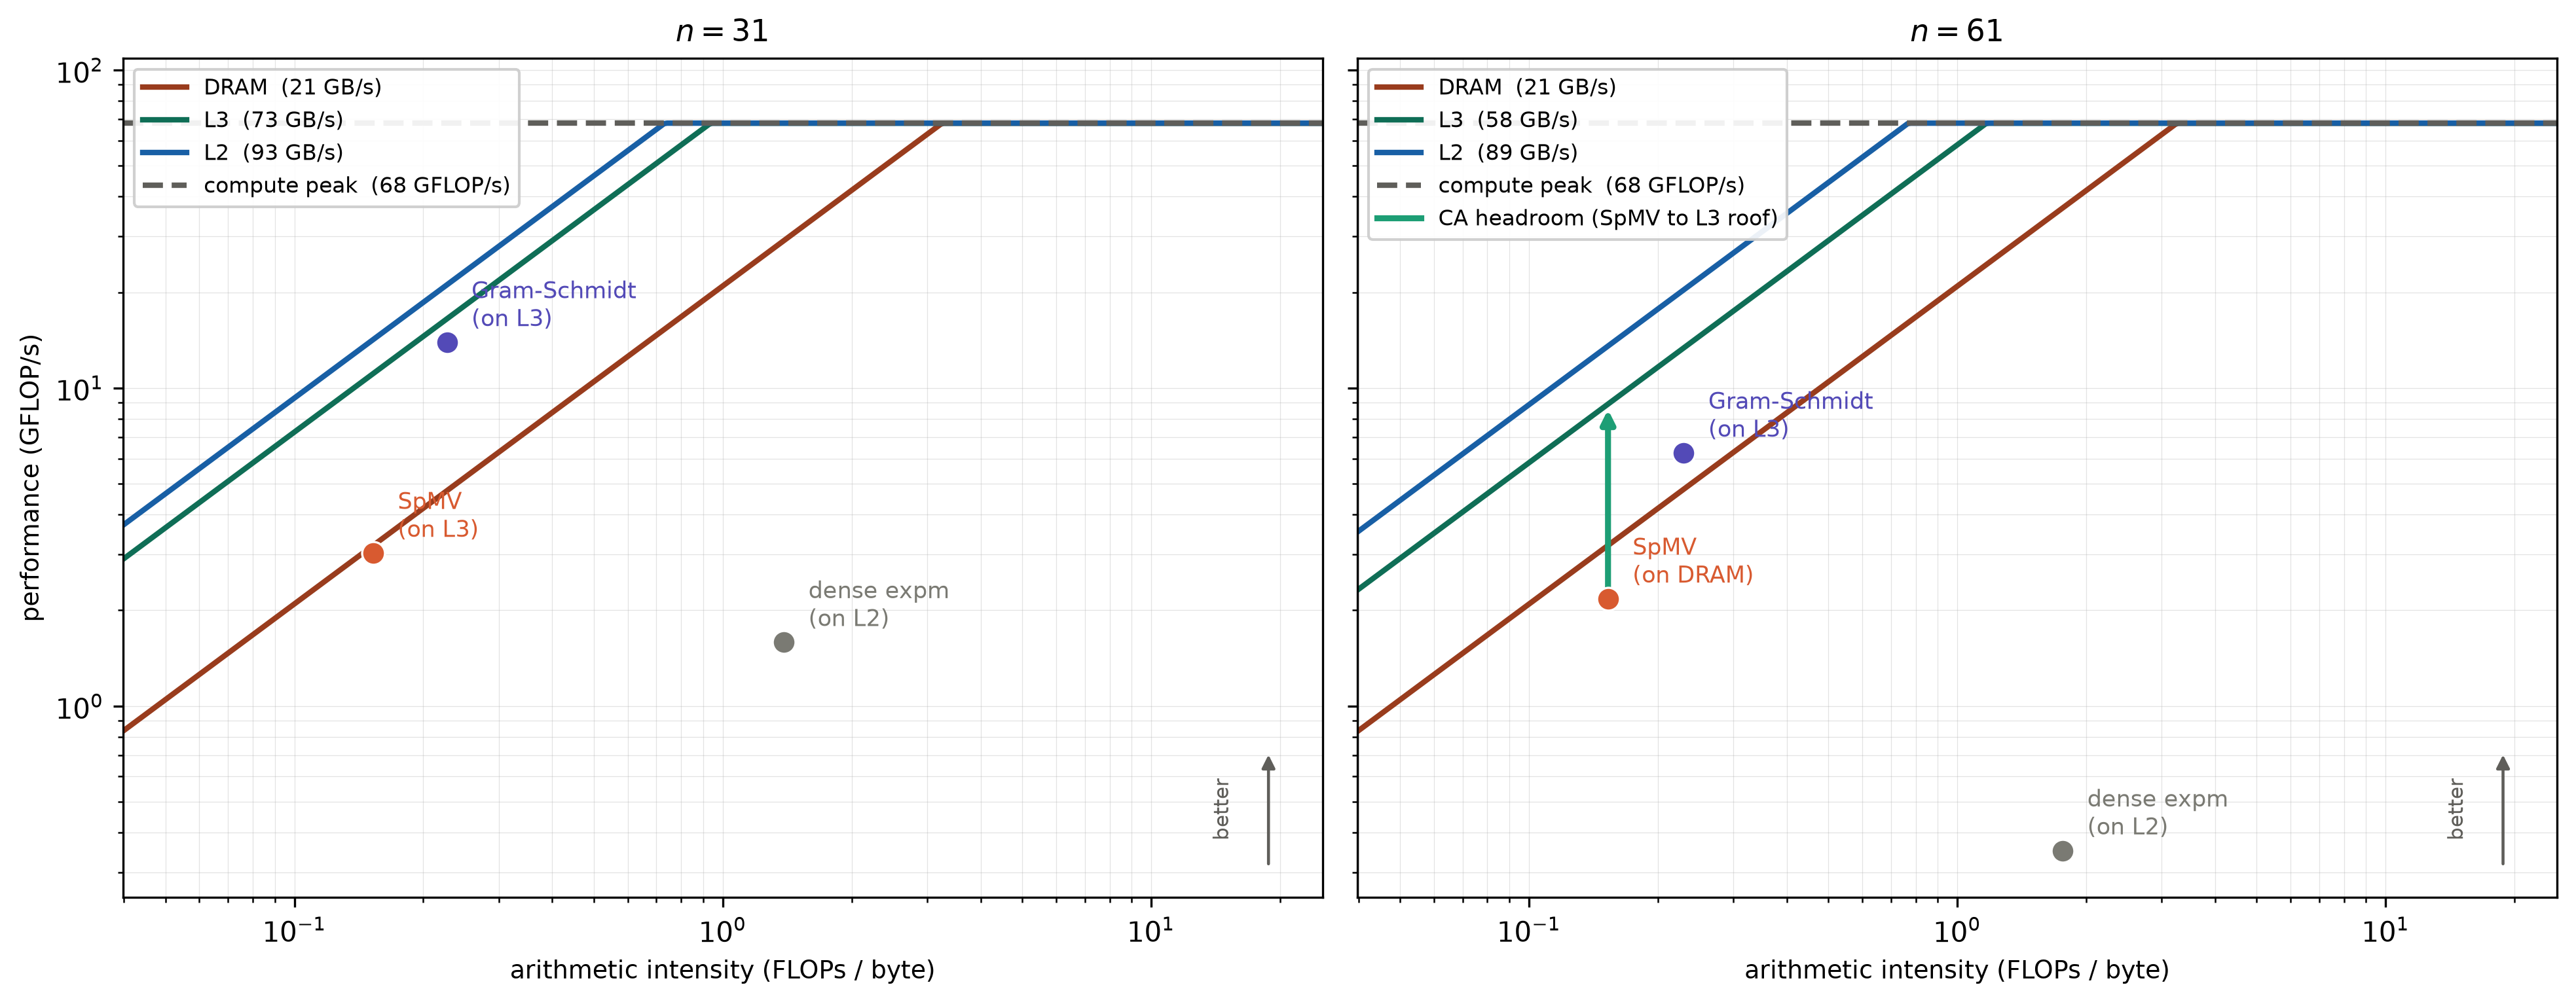
\includegraphics[width=0.9\textwidth]{cache_roofline.png}
\caption{Cache-aware roofline for the two hot kernels at $n=31$ and $n=61$. At $n=61$ the
SpMV has spilled to DRAM; the vertical distance from the measured point to the L3 roof at
the same arithmetic intensity is exactly the traffic a matrix-powers reformulation would
recover.}
\label{fig:roofline}
\end{figure}

\begin{table}[htbp]
\centering
\caption{Measured kernel positions on the roofline. AI is arithmetic intensity.}
\label{tab:roofline}
\begin{tabular}{@{}llccc@{}}
\toprule
\textbf{Grid} & \textbf{Kernel} & \textbf{AI (FLOP/B)} & \textbf{Achieved (GFLOP/s)} & \textbf{Resident tier} \\
\midrule
$n=31$ & SpMV          & 0.153 & 3.02  & L3 \\
$n=31$ & Gram--Schmidt & 0.227 & 13.91 & L3 \\
$n=61$ & SpMV          & 0.153 & 2.17  & \textbf{DRAM} \\
$n=61$ & Gram--Schmidt & 0.230 & 6.24  & L3 \\
\bottomrule
\end{tabular}
\end{table}

The attainable gain from moving a kernel one tier up the hierarchy is
\begin{equation}
\text{gain} = \frac{\min(BW_{\text{fast}} \cdot AI,\ \text{peak})}
                   {\min(BW_{\text{slow}} \cdot AI,\ \text{peak})},
\label{eq:gain}
\end{equation}
which collapses to the bandwidth ratio only while \emph{both} roofs are still sloped. It
must bend down once the fast roof reaches the compute ceiling---which the
$s\times$-higher arithmetic intensity of a matrix-powers kernel can actually reach.
Quoting a flat bandwidth ratio as ``the CA speedup'' overstates the ceiling.

%%%%%%%%%%%%%%%%%%%%%%%%%%%%%%%%%%%%%%%%%%%%%%%%%%%%%%%%%%%%%%%%%%%%%%%%%%%%%%%%%%%
\section{The OpenMP scaling study}\label{sec:scaling}

The scaling study measures how the two hot kernels of one Arnoldi cycle respond to added
cores---it does not measure solution accuracy. The thesis of the experiment is that the two
kernels fail to scale for two \emph{different} reasons, each motivating a distinct CA
mechanism (\Cref{tab:two-mechanisms}); this split is what the regime analysis of
\Cref{sec:regime} later turns into two independent dimensionless axes.

\subsection{Instrument design}

To make both ceilings visible and attributable, the harness freezes the Krylov dimension at
$m = 8$ with the convergence check disabled, so the Gram--Schmidt/SpMV work ratio does not
drift and any runtime change across the core count $P$ is attributable to hardware rather
than a changing algorithm (the genuine $m(n)$ growth is measured separately). It uses a
hand-rolled CSR, row-partitioned SpMV in which each thread is the sole writer of a
contiguous, disjoint slice of the output vector, with partition seams aligned to the cache
line; it runs MGS with parallel global reductions, exposing the synchronization cost
directly; and it reports per-kernel timings so a single sweep yields SpMV's plateau and
Gram--Schmidt's roll-off on one axis. Runs pin threads with \texttt{OMP\_PLACES=cores} and
\texttt{OMP\_PROC\_BIND=close}, so each CCX fills before the next engages and per-CCX L3
bandwidth steps appear as discrete risers; the swept core counts are CCX-boundary aligned
and SMT lanes are excluded. Each point is the median of five to seven timed repeats after a
warm-up, with the inter-quartile range as the error bar.

Two initialization arms form a controlled A/B experiment on memory placement: arm A fills
the matrix from thread 0 (first-touch parks it on one memory placement), arm B has each
thread first-touch exactly the row partition it will later compute on. The two arms turn
out to be indistinguishable---for a reason that is itself the finding, taken up in
\Cref{sec:locality}.

\begin{figure}[htbp]
\centering

\includegraphics[width=\textwidth]{scaling_strong.png}
\caption{Per-kernel strong scaling at $n=31$ and $n=61$, both initialization arms. SpMV
shows a plateau at $n=31$ and a superlinear transition at $n=61$; Gram--Schmidt shows the
synchronization staircase.}
\label{fig:strong}
\end{figure}

\begin{figure}[htbp]
\centering

\includegraphics[width=\textwidth]{scaling_weak.png}
\caption{Per-kernel weak-scaling efficiency $T(1)/T(P)$ with $n(P) = n_1 P^{1/3}$ rounded
odd, cache-tier crossings annotated.}
\label{fig:weak}
\end{figure}

\subsection{The quarantined $m(n)$ growth}

The harness freezes $m$ so that the scaling curves measure hardware; the genuine growth of
the Krylov dimension with the grid is measured separately and reported as an independent
numerical-analysis finding (\Cref{fig:mn}). The mean $\bar m$ per step grows from 7.6 at
$n=31$ to 11.3 at $n=89$---slow growth, but enough to drive Gram--Schmidt's quadratic
share upward (\Cref{tab:profile}), and the input to the small-$m$ safety argument of
\Cref{sec:ledger}.

\begin{figure}[htbp]
\centering

\includegraphics[width=0.85\textwidth]{scaling_mn.png}
\caption{The $m(n)$ Krylov-growth curve, measured with the convergence check enabled and
quarantined from the scaling instrument, which pins $m=8$.}
\label{fig:mn}
\end{figure}

\subsection{Why the transition happens: the locality control}\label{sec:locality}

At $n = 61$ the SpMV runtime drops \emph{superlinearly} (36.7$\times$ on 24 cores) with a
knee at $P = 12$ (\Cref{fig:strong}). The hypothesis: once each CCX's share of the matrix
($3 \times 52.8/P$\,MiB) fits in its own 16\,MiB L3 slice and stays resident across the
repeated SpMVs, reads come from L3 instead of DRAM. Quantitatively this checks out---the
implied aggregate bandwidth crosses the socket DRAM ceiling (${\sim}95$\,GB/s) exactly at
$P=12$, which is impossible from DRAM and therefore proves L3 residency.

The initialization arms \emph{cannot} test this: the 3960X is single-NUMA, and Zen~2 L3 is
a per-CCX victim cache, so L3 residency is set by which core \emph{accesses} a row, not by
which thread first-touched the page. Both arms use the same row partition and produce
identical curves. The real controlled experiment is over the \emph{compute schedule}, which
changes only which rows each core reads (\Cref{tab:locality}, \Cref{fig:locality}).

\begin{table}[htbp]
\centering
\caption{The locality control at $n=61$: three compute schedules, their predictions, and
the measurements (SpMV speedup at $P=24$; implied aggregate bandwidth at $P=12$).}
\label{tab:locality}
\begin{tabular}{@{}lp{4.2cm}p{4.3cm}p{4.3cm}@{}}
\toprule
\textbf{Schedule} & \textbf{What it does} & \textbf{Prediction} & \textbf{Measured} \\
\midrule
\texttt{block}  & contiguous band per core, fixed across SpMVs & transition at $P=12$ (locality-preserving control) & \textbf{confirmed}: 36.7$\times$, knee at $P=12$, 176\,GB/s \\
\texttt{cyclic} & cache-line blocks dealt round-robin, fixed & still transitions---scatter leaves per-CCX \emph{volume} unchanged & \textbf{refuted}: 7.0$\times$, no knee, 36\,GB/s \\
\texttt{rotate} & contiguous bands, rotating by one each SpMV & transition vanishes---no CCX retains a cache-fitting subset & \textbf{confirmed}: 6.6$\times$, no knee, 66\,GB/s \\
\bottomrule
\end{tabular}
\end{table}

\begin{figure}[htbp]
\centering

\includegraphics[width=0.95\textwidth]{scaling_locality.png}
\caption{The locality control. Only \texttt{block} carries an aggregate bandwidth DRAM
cannot supply, so the transition is genuinely L3 residency, not a scheduling coincidence.}
\label{fig:locality}
\end{figure}

The refuted \texttt{cyclic} prediction is a result in its own right, and it sharpens the CA
argument. Per-CCX \emph{volume} is not sufficient for residency: dealing cache-line blocks
round-robin leaves each CCX holding the same number of bytes scattered across the whole
matrix, and the arm collapses to roughly the \texttt{rotate} curve (7.0$\times$ vs.\
6.6$\times$) rather than the \texttt{block} one (36.7$\times$). \textbf{Contiguity, not
volume, is what keeps a slice resident}---which is exactly the property a matrix-powers
tiling is built to exploit, and exactly the property the scattered arm of the vertical
sweep (\Cref{sec:vertical}) destroys on purpose. The identical arm-A/arm-B result thereby
stops being an embarrassment and becomes the control that establishes the transition as a
locality effect---the ``before'' that the CA matrix-powers reformulation improves on.

%%%%%%%%%%%%%%%%%%%%%%%%%%%%%%%%%%%%%%%%%%%%%%%%%%%%%%%%%%%%%%%%%%%%%%%%%%%%%%%%%%%
\section{Regime analysis: a dimensionless map}\label{sec:regime}

The scaling study says the baseline solver is memory-bound and synchronization-bound. It
does not say whether a CA reformulation would \emph{help}, or where. The regime analysis
answers that with a dimensionless map whose two axes are the two mechanisms, with a
predicted crossover at 1 on each, plus a synthetic instrument that can be dialed to any
point on the map and a real Black--Scholes operator that is \emph{placed} on it by
measurement.

The non-circularity rule of \Cref{sec:intro} is enforced structurally: the predictor lives
in a header that never sees a timer (\texttt{regime.hpp}). In particular, $\Rh$'s
numerator is a machine constant times a tree depth, never a measured fraction of runtime.

\subsection{The coordinates}\label{sec:coords}

\begin{table}[htbp]
\centering
\caption{The two dimensionless coordinates.}
\label{tab:coords}
\begin{tabular}{@{}lp{5.2cm}p{4.6cm}l@{}}
\toprule
\textbf{Axis} & \textbf{Definition} & \textbf{Mechanism it governs} & \textbf{Scales like} \\
\midrule
$\Rv$ & Arnoldi working set / aggregate last-level cache & \textbf{vertical}: matrix-powers tiling, avoiding DRAM traffic & ${\sim}1/P$ \\
$\Rh$ & reduction cost / compute per core between reductions & \textbf{horizontal}: $s$-step, cutting the reduction count & ${\sim}P\log P$ \\
\bottomrule
\end{tabular}
\end{table}

Both crossovers are predicted at $R = 1$ ($\theta_v = \theta_h = 1$), giving four corners:
neither mechanism (lower-left), horizontal only (lower-right), vertical only (upper-left),
and both (upper-right). The Krylov dimension $m$ was demoted from an axis to a
\emph{modulator}: it moves working sets, so it moves $\Rv$, but it is not itself a portable
coordinate---two machines with the same $m$ can sit on opposite sides of $\theta_v$.

$\Rh$'s numerator needs a magnitude, not just a shape in $P$, or $\theta_h$ cannot be drawn
at all. A calibration instrument measures it directly as a bare scalar all-reduce over an
empty team---no payload, no application---and the model fitted to it is
\begin{equation}
t_{\text{reduce}}(P) = t_{\text{intra}} \cdot \text{intra levels}(P)
  + t_{\text{cross}} \cdot \min(\text{cross levels}(P),\ L^{*}).
\label{eq:treduce}
\end{equation}
On puffin: $t_{\text{intra}} = 120.8$\,ns, $t_{\text{cross}} = 652.8$\,ns (a cross-CCX tree
level costs 5.4$\times$ an intra-CCX one), and $L^{*} = 2.20$---past roughly two
cache-domain crossings, subtree concurrency hides the rest. Measured tree all-reduce
latency runs from 9.6\,ns at $P=1$ to 1.70\,$\mu$s at $P=24$ ($R^2 = 0.98$ against the
model). The cost is set by how many cache-domain boundaries the tree crosses, not by core
count---which is precisely why this coordinate cannot be measured on a virtualized
topology (\Cref{sec:platform}).

\subsection{The instrument and its gates}\label{sec:gates}

The numerics gate is not a timing run: nothing is threaded or timed, and no result depends
on the host. It establishes that the synthetic instrument's a-priori arithmetic predictions
hold before any communication claim is built on them (\Cref{tab:gates}).

\begin{table}[htbp]
\centering
\caption{The controls. A gate failure is fatal to everything downstream; a finding is a
result in its own right.}
\label{tab:gates}
\begin{tabular}{@{}lp{9.2cm}l@{}}
\toprule
\textbf{Control} & \textbf{Claim under test} & \textbf{Status} \\
\midrule
C1  & the Kronecker-sum spectrum is analytic and correct & gate \\
C2  & the scatter knob is an exact similarity transform (so a pure-$\Rv$ dial exists) & gate \\
C3  & measured $m$ obeys the Hochbruck--Lubich spectral bound \cite{hochbruck-lubich-1997} & gate (Hermitian PSD) \\
C3b & a spectral shift leaves $m$ fixed & finding \\
C4  & $\kappa$ of the matrix-powers basis equals the row-scaled Vandermonde from the spectrum & gate when normal \\
C5  & the CholeskyQR certificate $\kappa \le u^{-1/2}$ \cite{yamamoto-2015} is sound & gate \\
C5b & worst-case block count over the physical ensemble (``small-$m$ safety'') & finding \\
C6  & where the operator is non-normal, does the spectral prediction survive? & finding \\
\bottomrule
\end{tabular}
\end{table}

C2 is load-bearing. The scatter knob permutes the operator symmetrically,
$\mat{P}\mat{A}\mat{P}^\top$, which moves bytes and provably nothing else; if it moved the
spectrum, the ``pure $\Rv$ line'' would be an illusion and every vertical result would be
confounded. The sweep runs in five phases---gate, confound, $m$-range, non-normal, and
finally the real discretized Black--Scholes operator with its actual discounted payoff,
swept across grids. That last phase is \emph{transfer by measurement}: it lands the real
operator on the same $(\Rv, \Rh)$ plane as the synthetic instrument.

\subsection{Basis conditioning and the confound control}\label{sec:conditioning}

The certified $s$-step block width $s_{\max}$ is predicted from the spectrum alone (a
row-scaled Vandermonde \cite{trefethen-1997}), then measured. Where a closed-form spectrum
exists the prediction is \textbf{integer-exact on 20 of 21 runs}; the single exception is
the most violently non-normal point in the sweep ($\gamma = 0.4$,
$\kappa(X) = 7.7 \times 10^8$) and is off by one step. Every deviation larger than that
lives in the variable-advection arm---the family the log-robustness law
(\Cref{sec:nonnormality}) explicitly excludes. The real Black--Scholes operator deviates by
at most one step at any grid measured (\Cref{fig:conditioning}).

\begin{figure}[htbp]
\centering
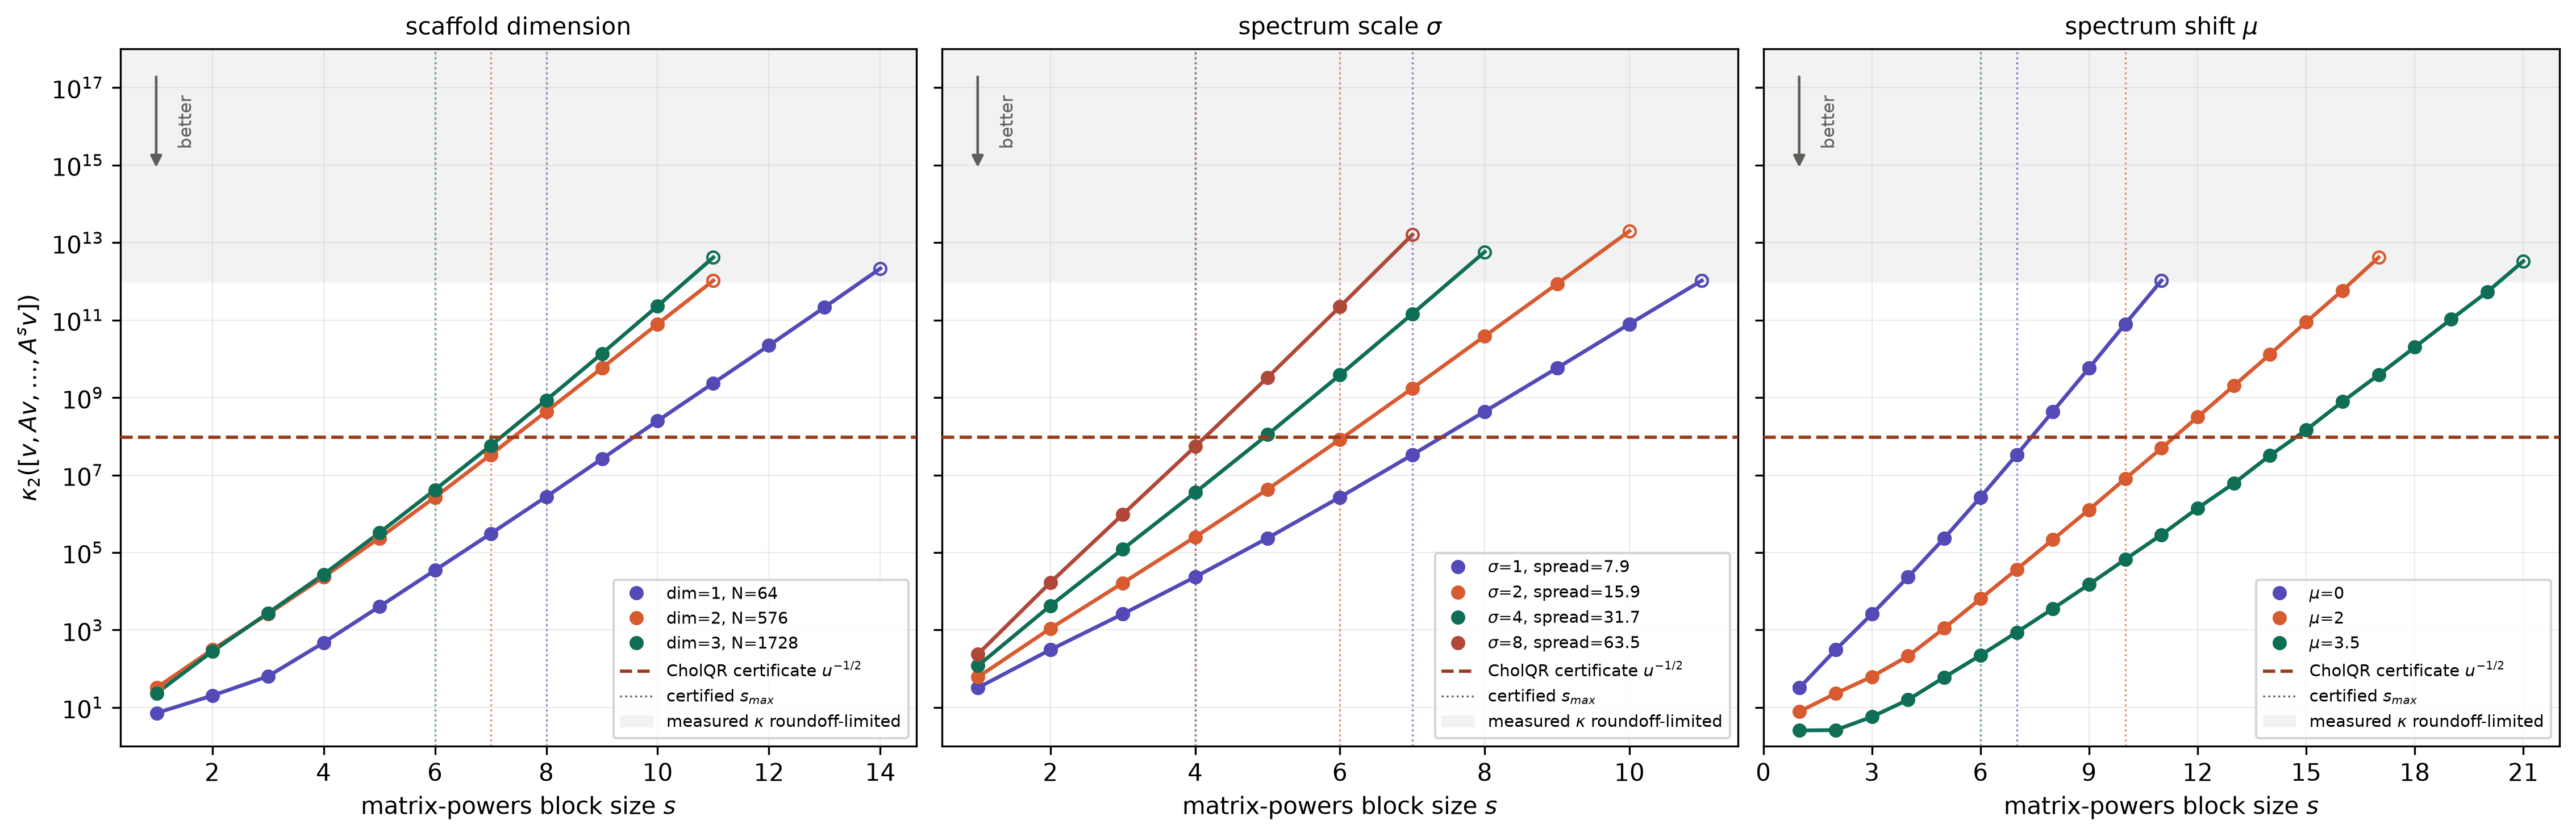
\includegraphics[width=0.95\textwidth]{regime_conditioning.png}
\caption{Predicted vs.\ measured basis condition number and the certified block width
$s_{\max}$ across the swept operator family.}
\label{fig:conditioning}
\end{figure}

The obvious confound is that $s_{\max}$ might just be tracking the Krylov dimension $m$. It
does not (\Cref{fig:confound}): with the spectrum pinned and $m$ moved through
$5\text{--}12$ (via the step size and tolerance), $s_{\max}$ stays flat at 7; with $m$
pinned at 5 and the spectrum scaled and shifted, $s_{\max}$ ranges from 4 to 14. Safety is
a property of the spectrum, not of the Krylov dimension.

\begin{figure}[htbp]
\centering
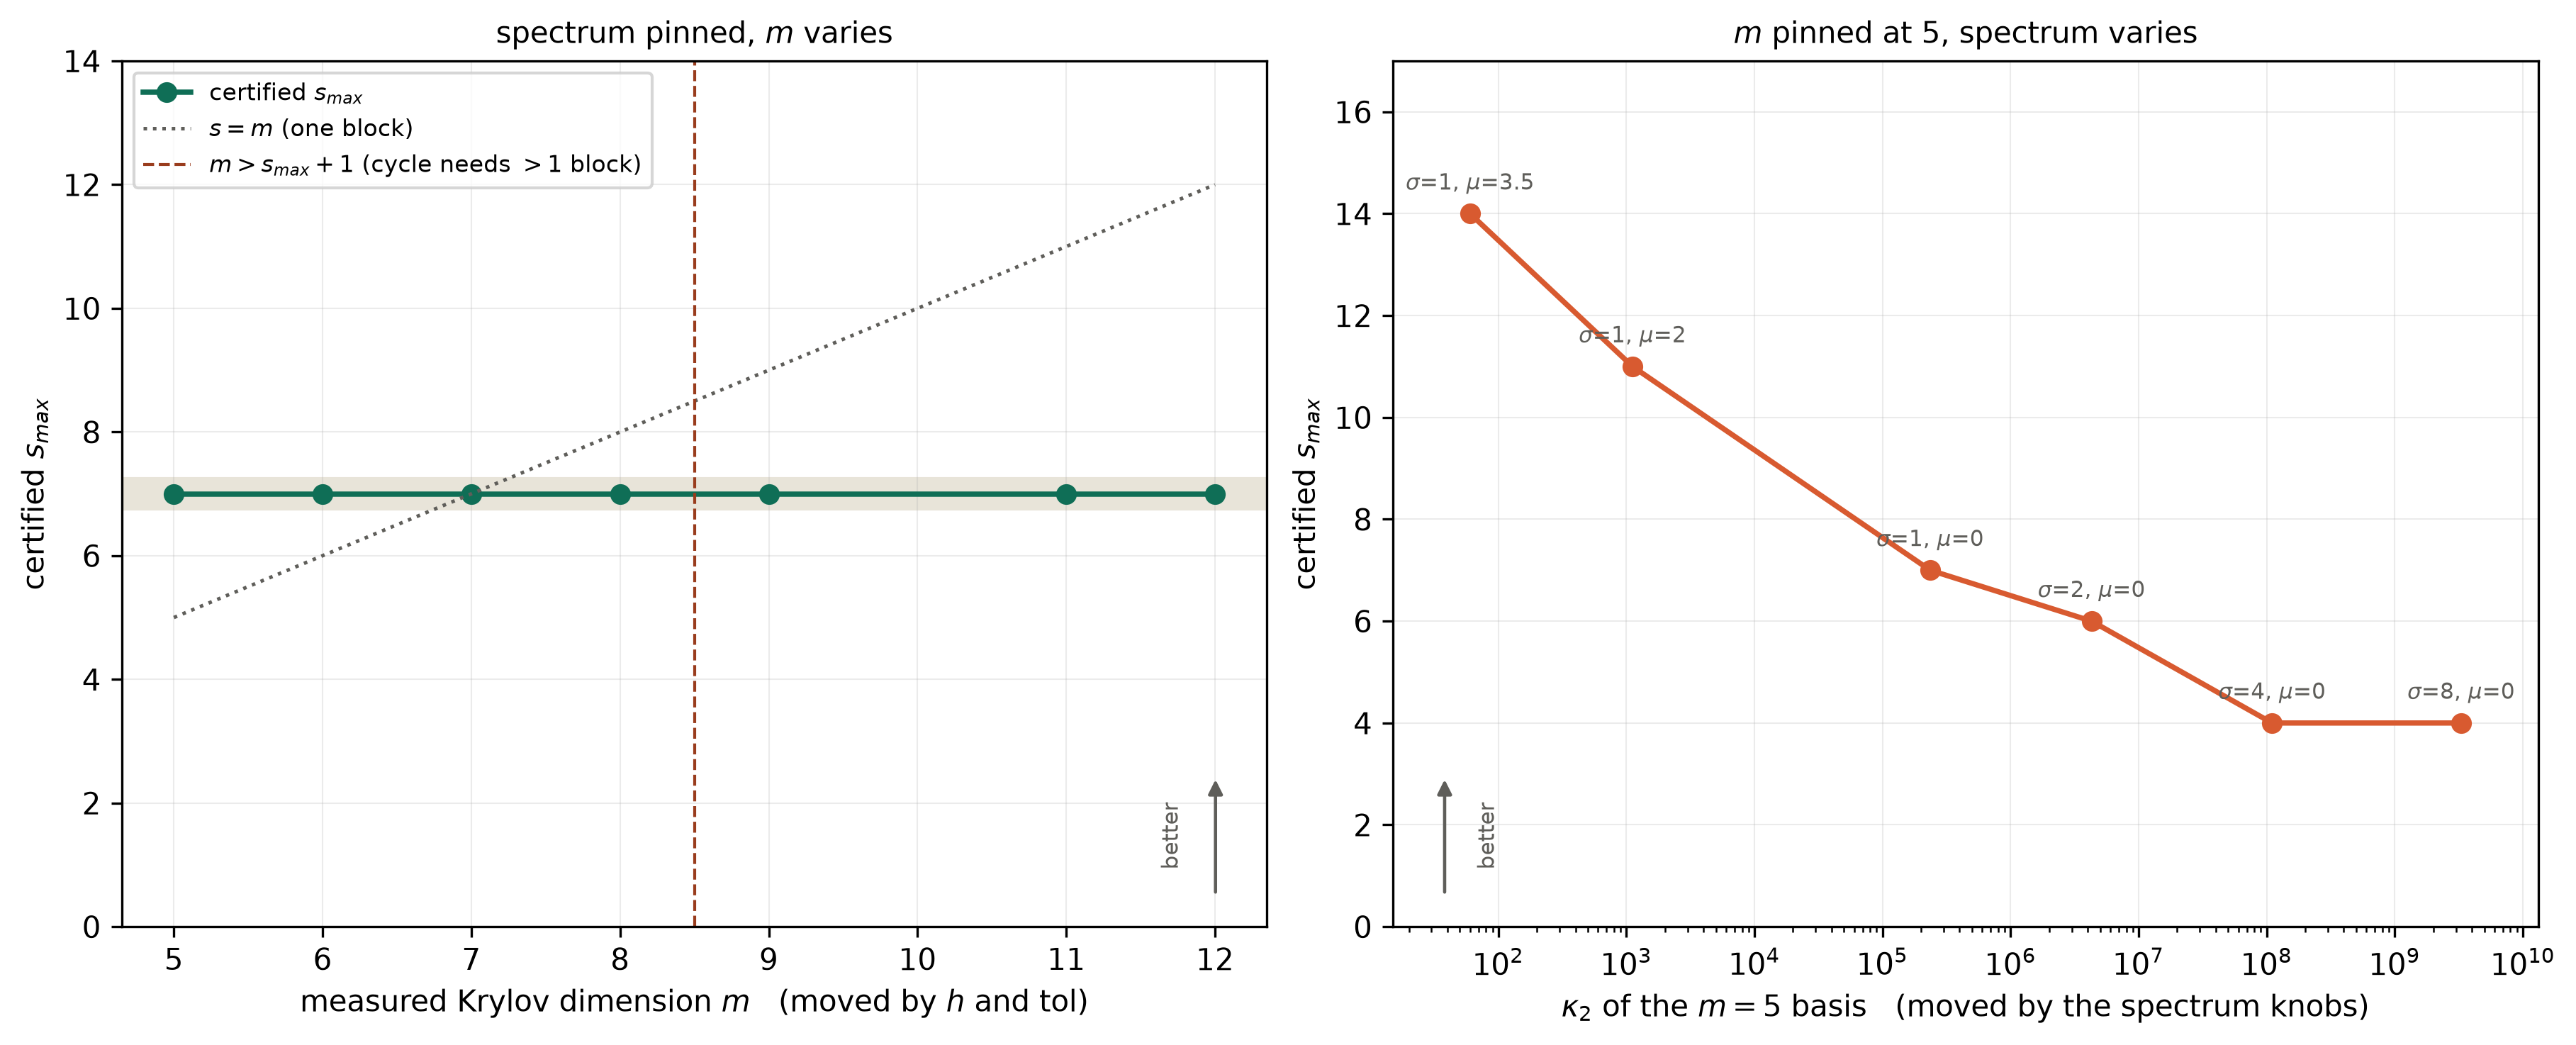
\includegraphics[width=0.95\textwidth]{regime_confound.png}
\caption{The confound control: $s_{\max}$ under pinned spectrum with varying $m$ (flat),
and pinned $m$ with varying spectrum (4--14).}
\label{fig:confound}
\end{figure}

\subsection{The reduction ledger and small-$m$ safety}\label{sec:ledger}

MGS performs $1 + m(m+3)/2$ global reductions per Arnoldi cycle. The stable $s$-step arm
(matrix powers + CholeskyQR2) performs $1 + 2\lceil m/(s_{\max}+1)\rceil$
(\Cref{tab:ledger}). Across the real problem's measured window $m = 8\text{--}11$ that is
an \textbf{11--16$\times$ cut in reduction count} at the $s_{\max} = 7$ certified for this
spectrum (\Cref{fig:reductions}).

\begin{table}[htbp]
\centering
\caption{The reduction ledger at $s_{\max} = 7$.}
\label{tab:ledger}
\begin{tabular}{@{}rrrr@{}}
\toprule
$m$ & \textbf{MGS reductions} & $s$\textbf{-step + CholQR2} & \textbf{cut} \\
\midrule
5  & 21 & 3 & 7.0$\times$ \\
8  & 45 & 3 & 15.0$\times$ \\
9  & 55 & 5 & 11.0$\times$ \\
11 & 78 & 5 & 15.6$\times$ \\
12 & 91 & 5 & 18.2$\times$ \\
\bottomrule
\end{tabular}
\end{table}

\begin{figure}[htbp]
\centering
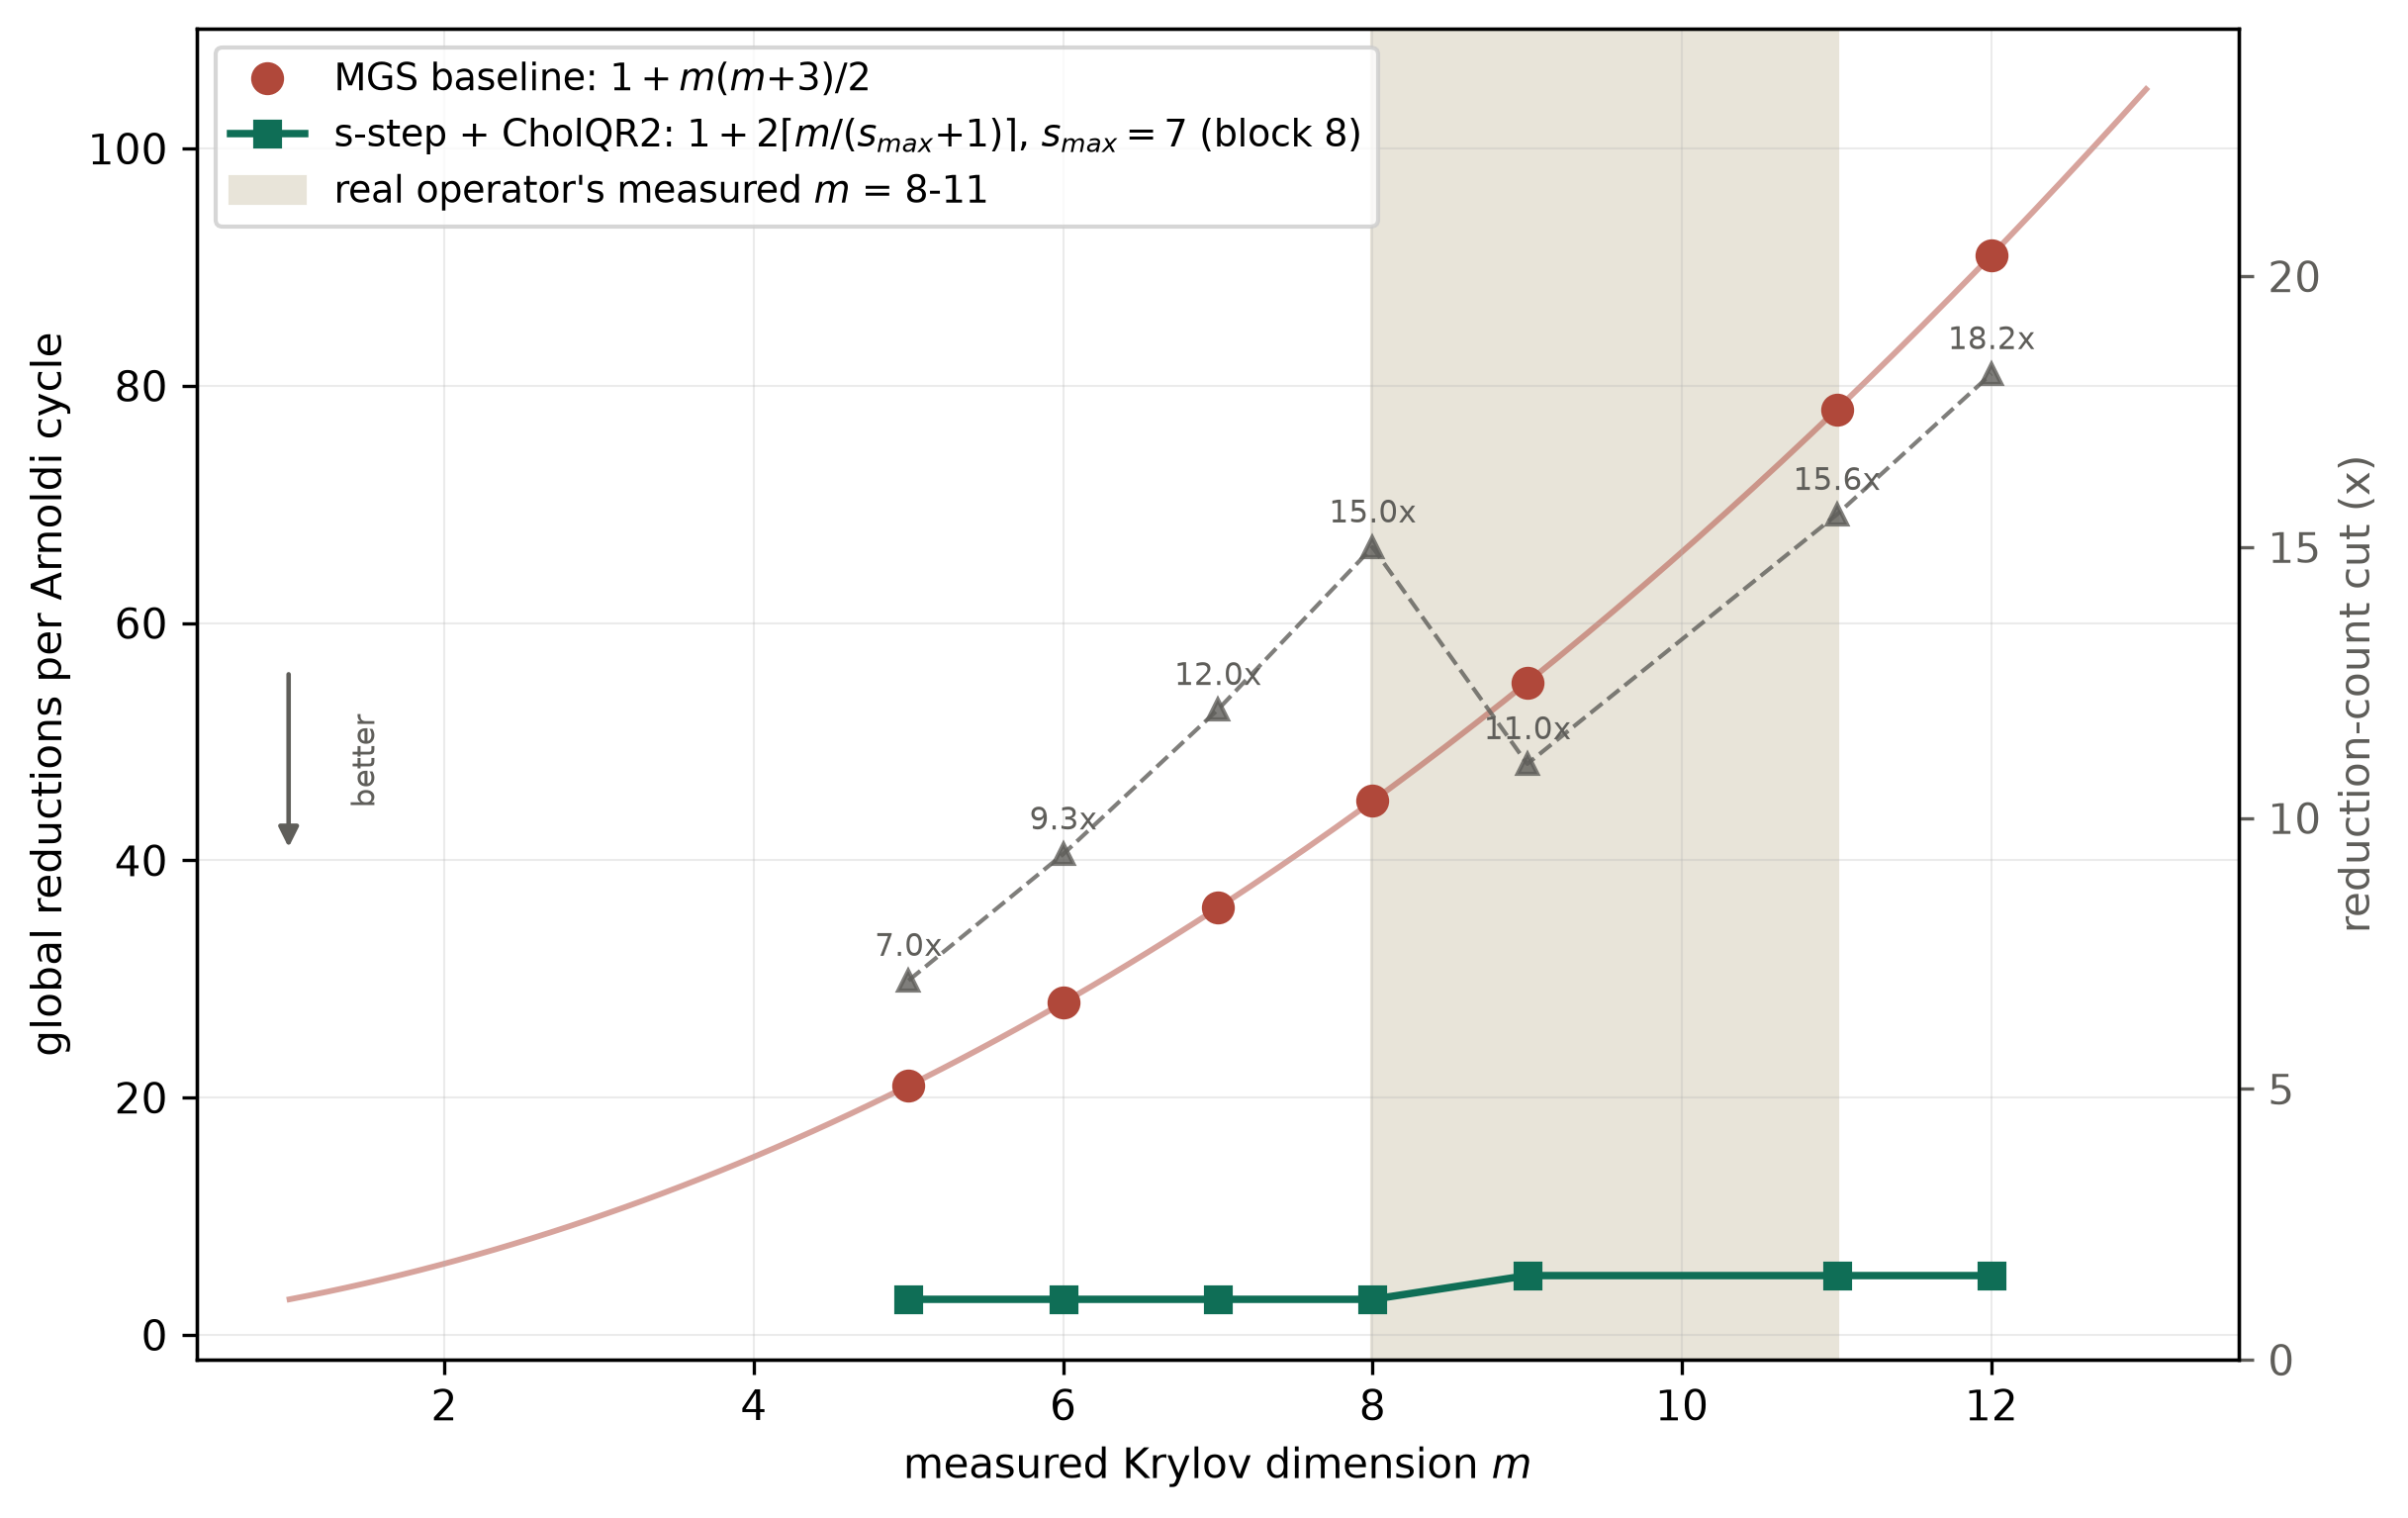
\includegraphics[width=0.9\textwidth]{regime_reductions.png}
\caption{Reductions per Arnoldi cycle: MGS vs.\ the certified $s$-step arm.}
\label{fig:reductions}
\end{figure}

\paragraph{Small-$m$ safety.} The real operator's Krylov dimension is small and grows
slowly: $m = 6\text{--}8$ across the eigensolvable grids $n = 10\text{--}20$, and 7.6 to
11.3 across $n = 31\text{--}89$ in production. Because a certified block yields
$s_{\max}+1$ vectors, an entire Arnoldi cycle fits in \textbf{2--3 blocks}. This is the
argument that makes $s$-step viable for this integrator at all: the machinery never has to
run deep enough for monomial-basis conditioning to become the dominant risk.

\subsection{Non-normality: the log-robustness law}\label{sec:nonnormality}

The spectral prediction of $s_{\max}$ assumes normality. The real operator is not normal
(mixed-derivative cross terms plus convection). The rigorous two-sided bound is that the
prediction error in decades is at most $\log_{10}\kappa(X)$, the eigenvector conditioning.
Measured, the data sits far below that line and grows only \emph{logarithmically}
(\Cref{fig:nonnormality}): the fitted slope of (error in decades) against
$\log_{10}\kappa(X)$ is \textbf{0.069} for the constant-coefficient mechanisms (advection,
correlation, and their combination) and \textbf{0.250}---about $4\times$ steeper---for
variable-coefficient advection (a position-dependent ramp). The two slopes differ by a
factor of four, so the law is \emph{scoped to the constant-coefficient family}, not
mechanism-independent---which is exactly why the variable-advection knob exists in the
instrument.

Both slopes are fitted on the canonical $\kappa(X)$ axis (\Cref{sec:dsweep}). This matters
for the constant-coefficient arm, whose zero-correlation half is a pure Kronecker sum: its
axes are interchangeable, so the dense $\kappa(X)$ there is degenerate and inflated by up
to $173\times$. Fitted on the dense axis the slope reads 0.061 instead of 0.069---small
enough not to disturb the conclusion, but the two arms would have been compared on axes of
different validity.

A \emph{decade} here is one factor of ten in the basis condition number; the unit is chosen
because it converts directly into block width. Each extra power appended to
$[\vect{v}, \mat{A}\vect{v}, \ldots, \mat{A}^s\vect{v}]$ multiplies its condition number by
a roughly constant factor, measured at a median of 1.05 decades per power over the swept
family (inter-quartile range 0.95 to 1.12), so the figure marks one $s$-step at 1.2
decades. An error below that line cannot move the certified block width by a full step.

The real Black--Scholes operator is placed on this figure as a test point, excluded from
every fit. Its prediction error runs 0.19 to 0.85 decades at $\kappa(X)$ up to
$2.3 \times 10^3$, comfortably \textbf{under one $s$-step} at every grid measured.

\begin{figure}[htbp]
\centering

\includegraphics[width=0.95\textwidth]{regime_nonnormality.png}
\caption{The log-robustness law: prediction error in decades vs.\ $\log_{10}\kappa(X)$.
The rigorous bound is the identity line; the measured data grows logarithmically, with the
constant-coefficient and variable-coefficient families fitted separately. The real
Black--Scholes operator (test point, excluded from fits) sits under one $s$-step at every
grid.}
\label{fig:nonnormality}
\end{figure}

Operator by operator, what the spectral prediction needs is normality; definiteness and
separability are conveniences (\Cref{tab:operators}).

\begin{table}[htbp]
\centering
\caption{Which structural properties the spectral prediction of $s_{\max}$ actually needs.}
\label{tab:operators}
\begin{tabular}{@{}lllll@{}}
\toprule
\textbf{Operator} & \textbf{Normal?} & \textbf{Definite?} & \textbf{Separable?} & \textbf{Spectral prediction} \\
\midrule
Laplacian                    & yes & PSD        & yes & exact (closed form) \\
shift $\mu$                  & yes & indefinite & yes & exact ($\kappa(X) = 1$) \\
correlation $\rho$           & yes & PSD        & no  & exact (dense eigensolve) \\
constant $\gamma$ advection  & no  & --         & yes & survives ($<$ 1 step) \\
$\rho + \gamma$              & no  & --         & no  & survives ($<$ 1 step) \\
variable $\gamma$ advection  & no  & --         & no  & must be measured ($>$ 1 step) \\
\bottomrule
\end{tabular}
\end{table}

\subsection{The asset-dimension law}\label{sec:dsweep}

How does $\kappa(X)$ grow with the number of assets $d$? This axis matters because the
application grows the asset count, not the grid: a refinement study swept the grid at fixed
$d = 3$ and found $\kappa(X)$ flat, which confirms the mesh-P\'eclet reading
($\log\kappa(X) \sim d\, n_1 \gamma$ with $\gamma \sim C/n_1$, so $n_1$ cancels) and says
nothing about $d$.

\textbf{The law is linear in $d$, with a slope known in closed form.} The synthetic
operator applies its cross term to exactly one axis pair at every $d$, so it factors as a
Kronecker sum $\mat{A}_d = \mat{B}_{01} \oplus \mat{T} \oplus \cdots \oplus \mat{T}$. A
Kronecker product multiplies singular values, so
\begin{equation}
\kappa(X) = \kappa(X_{01})\, \kappa(X_1)^{\,d-2}
\qquad\Longrightarrow\qquad
\log_{10}\kappa(X) = 0.40499\, d + 0.01422,
\label{eq:tensor-law}
\end{equation}
with the slope $0.404995 = \log_{10}\kappa(X_1)$ analytic. The observed $d = 2 \to 3$
increment is $0.40500$, and the formula reproduces both degeneracy-free points to
$3 \times 10^{-7}$.

The dense $\kappa(X)$ that a straightforward eigensolve returns must \emph{not} be fitted
along $d$, because from $d = 4$ it is not a property of the operator at all. Axes
$2, \ldots, d-1$ carry no cross term, so interchanging any two of them is an exact symmetry
of $\mat{A}$: the spectrum repeats, and inside a repeated eigenspace every basis is
admissible, so the value reported is whichever basis the eigensolver's rounding happened to
produce. A symmetric permutation $\mat{P}\mat{A}\mat{P}^{\top}$ is an exact similarity, so
any function of the operator is invariant under it---yet the dense value moves by a factor
of 3.84 at $d = 4$ and 7.76 at $d = 5$ across eight permutations once the spectrum is
degenerate. The study therefore reports a canonical, basis-independent value
(\texttt{kappa\_X\_struct}, computed per Kronecker factor) alongside the dense one
(\Cref{tab:dsweep}, \Cref{fig:dsweep}).

\begin{table}[htbp]
\centering
\caption{Canonical vs.\ dense $\kappa(X)$ along the asset dimension.}
\label{tab:dsweep}
\begin{tabular}{@{}rrrrl@{}}
\toprule
$d$ & $N$ & \textbf{canonical} $\kappa(X)$ & \textbf{dense} $\kappa(X)$ & \textbf{spectrum} \\
\midrule
2 & 16   & 6.671 & 6.671            & simple (agree to $3\times 10^{-7}$) \\
3 & 64   & 16.95 & 16.95            & simple (agree to $3\times 10^{-7}$) \\
4 & 256  & 43.07 & 109.5            & degenerate: dense meaningless \\
5 & 1024 & 109.4 & $5.2\times 10^3$ & degenerate: dense meaningless \\
6 & 4096 & 278.1 & $3.7\times 10^4$ & degenerate: dense meaningless \\
\bottomrule
\end{tabular}
\end{table}

\begin{figure}[htbp]
\centering
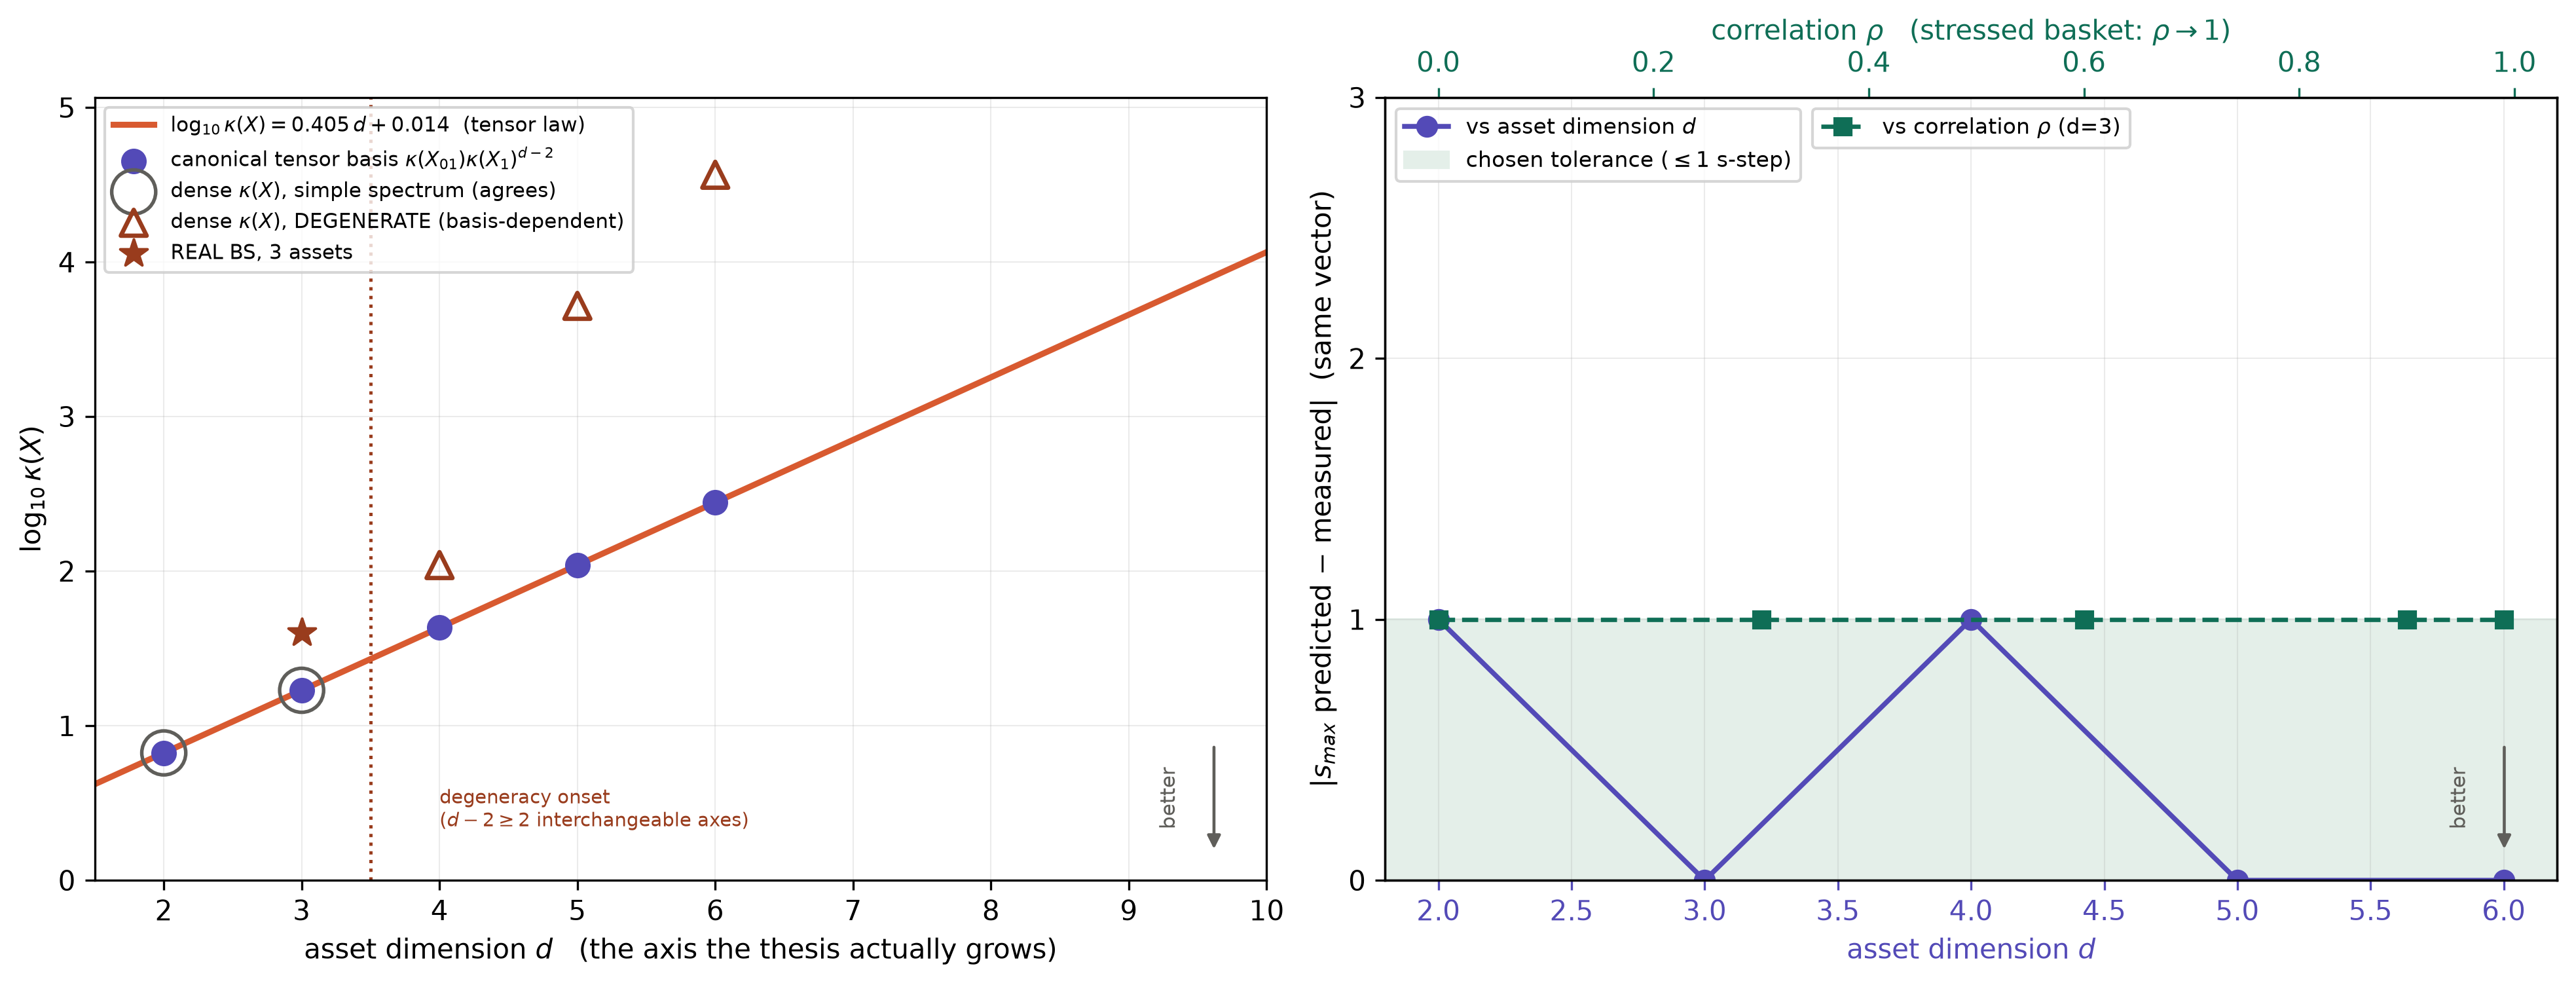
\includegraphics[width=0.95\textwidth]{regime_dsweep.png}
\caption{The asset-dimension law: canonical $\kappa(X)$ grows geometrically in $d$ with an
analytic slope; the dense value diverges from it exactly where the spectrum degenerates.}
\label{fig:dsweep}
\end{figure}

The correlation arm ($n_1 = 8$, $d = 3$) is sound wherever the cross term is actually
present, and its $\rho = 0$ endpoint is the most degenerate point in the study (only 89 of
512 eigenvalues distinct). With the canonical value as anchor (\Cref{tab:corr}),
\textbf{correlation raises $\kappa(X)$ monotonically}, from 688 at $\rho = 0$ to 3405 at
$\rho = 0.99$---about $5\times$ across the full range.

\begin{table}[htbp]
\centering
\caption{The correlation arm ($n_1 = 8$, $d = 3$). At $\rho > 0$ the dense value matches
the canonical one exactly; at $\rho = 0$ the operator is a pure Kronecker sum and the dense
value is degenerate.}
\label{tab:corr}
\begin{tabular}{@{}lrrrrr@{}}
\toprule
$\rho$ & 0 & 0.3 & 0.6 & 0.9 & 0.99 \\
\midrule
canonical $\kappa(X)$ & \textbf{688.0} & 851.8 & 1566.9 & 2277.9 & 3405.2 \\
dense $\kappa(X)$     & \emph{11350}   & 851.8 & 1566.9 & 2277.9 & 3405.2 \\
\bottomrule
\end{tabular}
\end{table} An earlier reading had correlation \emph{reducing}
$\kappa(X)$, but that took the degenerate $\rho = 0$ dense value ($1.14 \times 10^4$) as
its anchor, and permuting that same operator returns anything from $4 \times 10^4$ to
$1.5 \times 10^6$: there was no fall to explain. Dimension still dominates---$\rho$ across
its entire admissible range buys about 1.7 assets' worth of conditioning, and $\rho \le 1$
while $d$ is unbounded---but correlation never helps.

The practical consequence: \textbf{measure the block width at high $d$ rather than trusting
a conservative a-priori bound}, because $\kappa(X)$ grows geometrically in $d$ while
staying flat under grid refinement. The law's scope is the synthetic instrument: the real
basket operator couples all three asset pairs, so the tensor identity, which rests on one
coupled pair, does not extend to it.

\subsection{The computability gap}\label{sec:gap}

The certificate is validated by dense eigensolve, which caps the control at
$N \le 32{,}768$, while the performance claims live at $N \sim 10^5$. The proposed bridge
was to exploit the constant-coefficient Toeplitz structure for an analytic spectrum,
avoiding the eigensolve entirely. \textbf{That route is closed.} The cross term factors
exactly as $c\,(\mat{D} \otimes \mat{D})$ with $\mat{D} = \operatorname{tridiag}(-1,0,+1)$
(verified to machine zero). A diagonal similarity $\operatorname{diag}(z^j)$ symmetrizes
$\operatorname{tridiag}(b, a, c)$ iff $z^2 = c/b$---and the two terms demand incompatible
$z$ on the same axis: $z^2 = (1-\gamma)/(1+\gamma)$ for advection--diffusion against
$z^2 = -1$ for the cross factor. Numerically, the sine basis leaves 3.7\% off-diagonal mass
with the cross term against $2.8 \times 10^{-14}$ without, and no single $z$ helps. The
obstruction persists at $\gamma = 0$, so it is the Dirichlet boundary condition, not the
advection.

The consolation is constructive: the tensor identity \eqref{eq:tensor-law} gives
$\kappa(X)$ at any $d$ from a single $n_1^2 \times n_1^2$ eigensolve---no $N \times N$
solve and no cap---\emph{for the synthetic operator}. The gap remains open for the real
Black--Scholes operator, whose all-pairs correlation breaks the Kronecker factorization.

\subsection{The horizontal mechanism: a measured null result}\label{sec:horizontal}

The reduction ledger promises an 11--16$\times$ cut in reduction \emph{count}. The
wall-clock does not move. Two independent measurements say why, and they agree:
\begin{enumerate}
\item \textbf{The primitive was never the bottleneck.} Replacing the naive
  barrier-plus-$O(P)$-scan reduction with a proper binary tree---a 1.7$\times$ improvement
  in the bare all-reduce latency at $P = 24$ (2.91\,$\mu$s down to 1.70\,$\mu$s)---leaves
  Gram--Schmidt wall-clock unchanged to within 5\% at every core count. The OpenMP
  runtime's barrier is already a tree, and the barrier itself dominates the scan.
\item \textbf{Gram--Schmidt is vector-bound, not reduction-bound.} MGS re-reads column
  $\vect{V}_i$ once for every $j \ge i$, so $m(m+1)/2$ column reads at $8N$ bytes each.
  That quadratic is a \emph{bandwidth} term, and it is what the roll-off in the scaling
  study is actually made of.
\end{enumerate}

\begin{figure}[htbp]
\centering

\includegraphics[width=0.9\textwidth]{scaling_reduction.png}
\caption{Gram--Schmidt wall-clock under the calibrated tree reduction vs.\ the $O(P)$
redundant scan it replaced ($n=61$, arm B; one contaminated $P=15$ launch, inflated across
all kernels, is excluded). A 1.7$\times$ faster primitive leaves the kernel unchanged
within 5\%.}
\label{fig:reduction}
\end{figure}

The map predicted this before the experiment: at production resolution $n = 61$ the real
operator sits at $\Rh = 0.080 \ll \theta_h = 1$. The horizontal mechanism has no home on
this machine, and the null result is a \emph{confirmation} of the coordinate, not a failure
of it. The thesis leads with the timed number, not the reduction count.

The upper-right corner---both mechanisms binding simultaneously---is structurally
unreachable on puffin. It is a single-NUMA socket, so no tree in the reduction crosses
anything more expensive than a CCX boundary; reaching $\theta_h$ at a working set that also
exceeds $\theta_v$ needs a reduction cost roughly 25$\times$ higher than any this machine
can produce.

\subsection{The vertical mechanism: a measured shortfall}\label{sec:vertical}

A timed sweep runs a cache-blocked matrix-powers kernel against the untiled baseline across
grids that carry $\Rv$ from 0.035 to 86. The modeled traffic ratio---the ceiling the
roofline says tiling could reach---is 4--8$\times$. The measurement is not close
(\Cref{tab:vertical}, \Cref{fig:sweep}).

\begin{table}[htbp]
\centering
\caption{The vertical sweep: measured speedup of the tiled matrix-powers kernel against
the modeled traffic ratio.}
\label{tab:vertical}
\begin{tabular}{@{}llccc@{}}
\toprule
\textbf{Pattern} & \textbf{Tile level} & $\Rv$ \textbf{(1 core)} & \textbf{Measured speedup} & \textbf{Modeled ratio} \\
\midrule
banded    & L3 & 0.035--2.69 & \textbf{0.72--1.31$\times$} & 4--8$\times$ \\
banded    & L2 & 1.12--86.1  & \textbf{0.37--0.89$\times$} & 4--8$\times$ \\
scattered & L3 & 0.035--2.69 & 1.00$\times$ (falls back to naive) & 4$\times$ \\
\bottomrule
\end{tabular}
\end{table}

\begin{figure}[htbp]
\centering
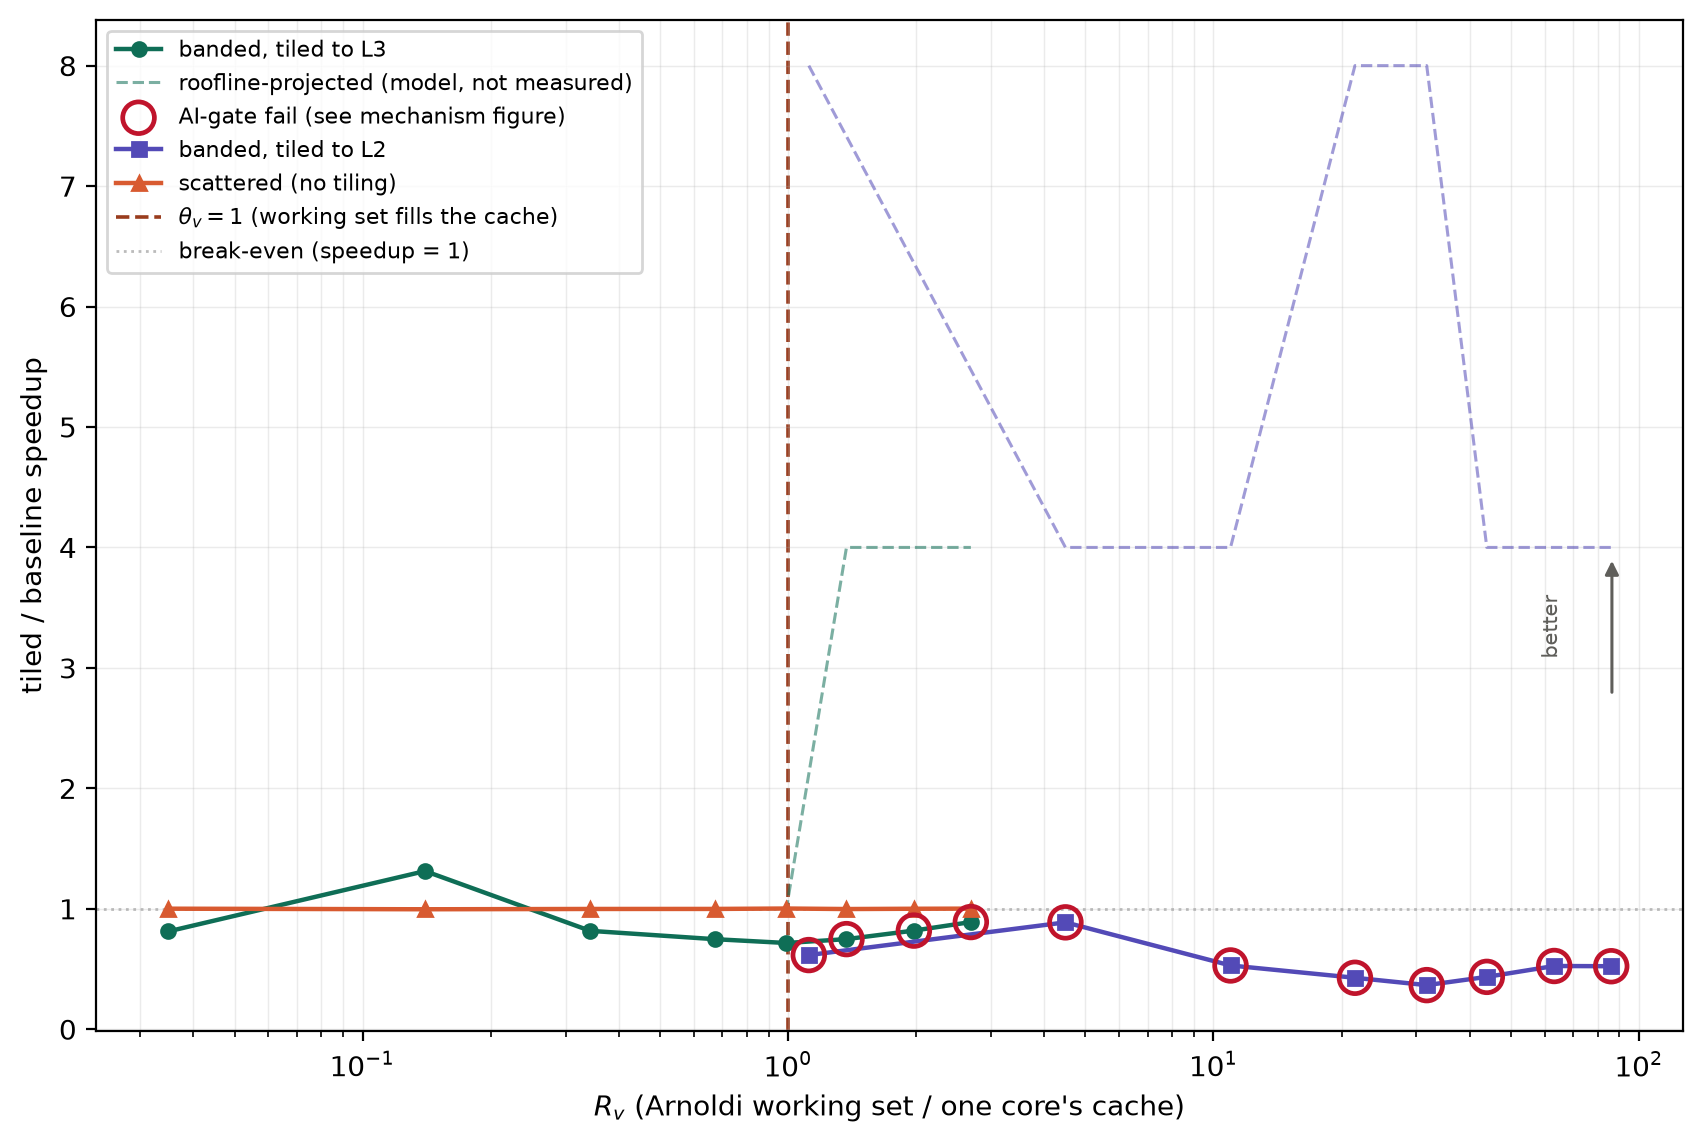
\includegraphics[width=0.95\textwidth]{regime_sweep.png}
\caption{The vertical sweep: measured speedup of cache-blocked matrix powers across
$\Rv$. The projected curve is an explicit model claim, drawn dashed, never presented as
data.}
\label{fig:sweep}
\end{figure}

This is a \textbf{kernel ceiling, not a refuted boundary}: the tiled arm never reached a
bandwidth-bound regime, so the experiment never got to test $\theta_v$. A diagnostic kernel
that skips the halo entirely (wrong basis, throughput only) separates the two tile levels
cleanly (\Cref{fig:mechanism}). At the L2 level (small panels, fat halo), removing the halo
recovers throughput toward baseline (1.17 rising to 2.13 against a 2.70 baseline at
$n_1 = 400$): cache-blocking \emph{works}, and the shortfall is redundant halo arithmetic
traded for DRAM traffic---a bad trade at these panel sizes, not a broken kernel. At the L3
level (large panels, thin halo), removing the halo barely moves throughput (2.06 to 2.11
against 2.76): neither arm is bandwidth-bound, and both are capped by something insensitive
to cache residency, most consistent with gather latency on the indirect column access.

\begin{figure}[htbp]
\centering

\includegraphics[width=0.95\textwidth]{regime_sweep_mechanism.png}
\caption{The no-halo diagnostic. L2 tiling recovers toward baseline without the halo (the
halo trade is the shortfall); L3 tiling barely moves (the cap is insensitive to cache
residency).}
\label{fig:mechanism}
\end{figure}

\textbf{The scattered arm delimits where the vertical mechanism cannot pay at all.}
Matrix-powers tiling is structurally impossible once the columns scatter, so the sweep
falls back to the naive form and measures 1.00$\times$ by construction. Since the scatter
knob is a similarity transform (gate C2), that boundary is a property of the sparsity
pattern alone, at fixed spectrum and fixed working set.

Two honest limitations. Nothing here is a \emph{counted} DRAM measurement, because
puffin's uncore counters need root, so modeled bytes are reconciled against the roofline
instead---weaker evidence, labeled as such on every figure. And the projected curve on
\Cref{fig:sweep} is a model claim, drawn dashed.

\subsection{Block width: two roofs, and which one binds}\label{sec:swidth}

Everywhere else the block width $s$ is pinned at the certified value, which hides a
question. $s$ is pushed \emph{up} by both mechanisms---a wider block means fewer reductions
and more powers per operator stream---and pulled \emph{down} by two independent ceilings:
\begin{itemize}
\item \textbf{numerical (the certificate):} $\kappa([\vect{v}, \mat{A}\vect{v}, \ldots,
  \mat{A}^s\vect{v}])$ grows geometrically in $s$; past $u^{-1/2}$ the monomial basis
  leaves the CholeskyQR certificate, so the block builds but will not orthogonalize.
\item \textbf{capacity (the ghost):} the halo is $s \cdot w$ rows per side, so a wider
  block shrinks the panel until none fits and the tiling collapses.
\end{itemize}
Which arrives first is a joint property of operator and machine, and on puffin it depends
on the tiling level (\Cref{tab:swidth}, \Cref{fig:swidth}).

\begin{table}[htbp]
\centering
\caption{The two roofs on the block width. The L3 ghost roof is quoted as $\ge$ because a
panel still fit at every swept $s$ up to the sweep ceiling of 24; the certificate roof is
measured directly ($\kappa(\mat{B}_s)$ crosses $u^{-1/2}$ between $s=8$ and $s=9$ at
$n_1 = 420$).}
\label{tab:swidth}
\begin{tabular}{@{}llccl@{}}
\toprule
\textbf{Tile level} & $n_1$ & \textbf{Certificate roof} $s$ & \textbf{Ghost roof} $s$ & \textbf{Binding roof} \\
\midrule
L3 & 420      & 8 & $\ge 24$ & \textbf{numerical} \\
L3 & 480, 560 & 6 & $\ge 24$ & \textbf{numerical} \\
L2 & 420      & 8 & 3        & \textbf{capacity} \\
L2 & 480      & 6 & 3        & \textbf{capacity} \\
L2 & 560      & 6 & 2        & \textbf{capacity} \\
\bottomrule
\end{tabular}
\end{table}

\begin{figure}[htbp]
\centering
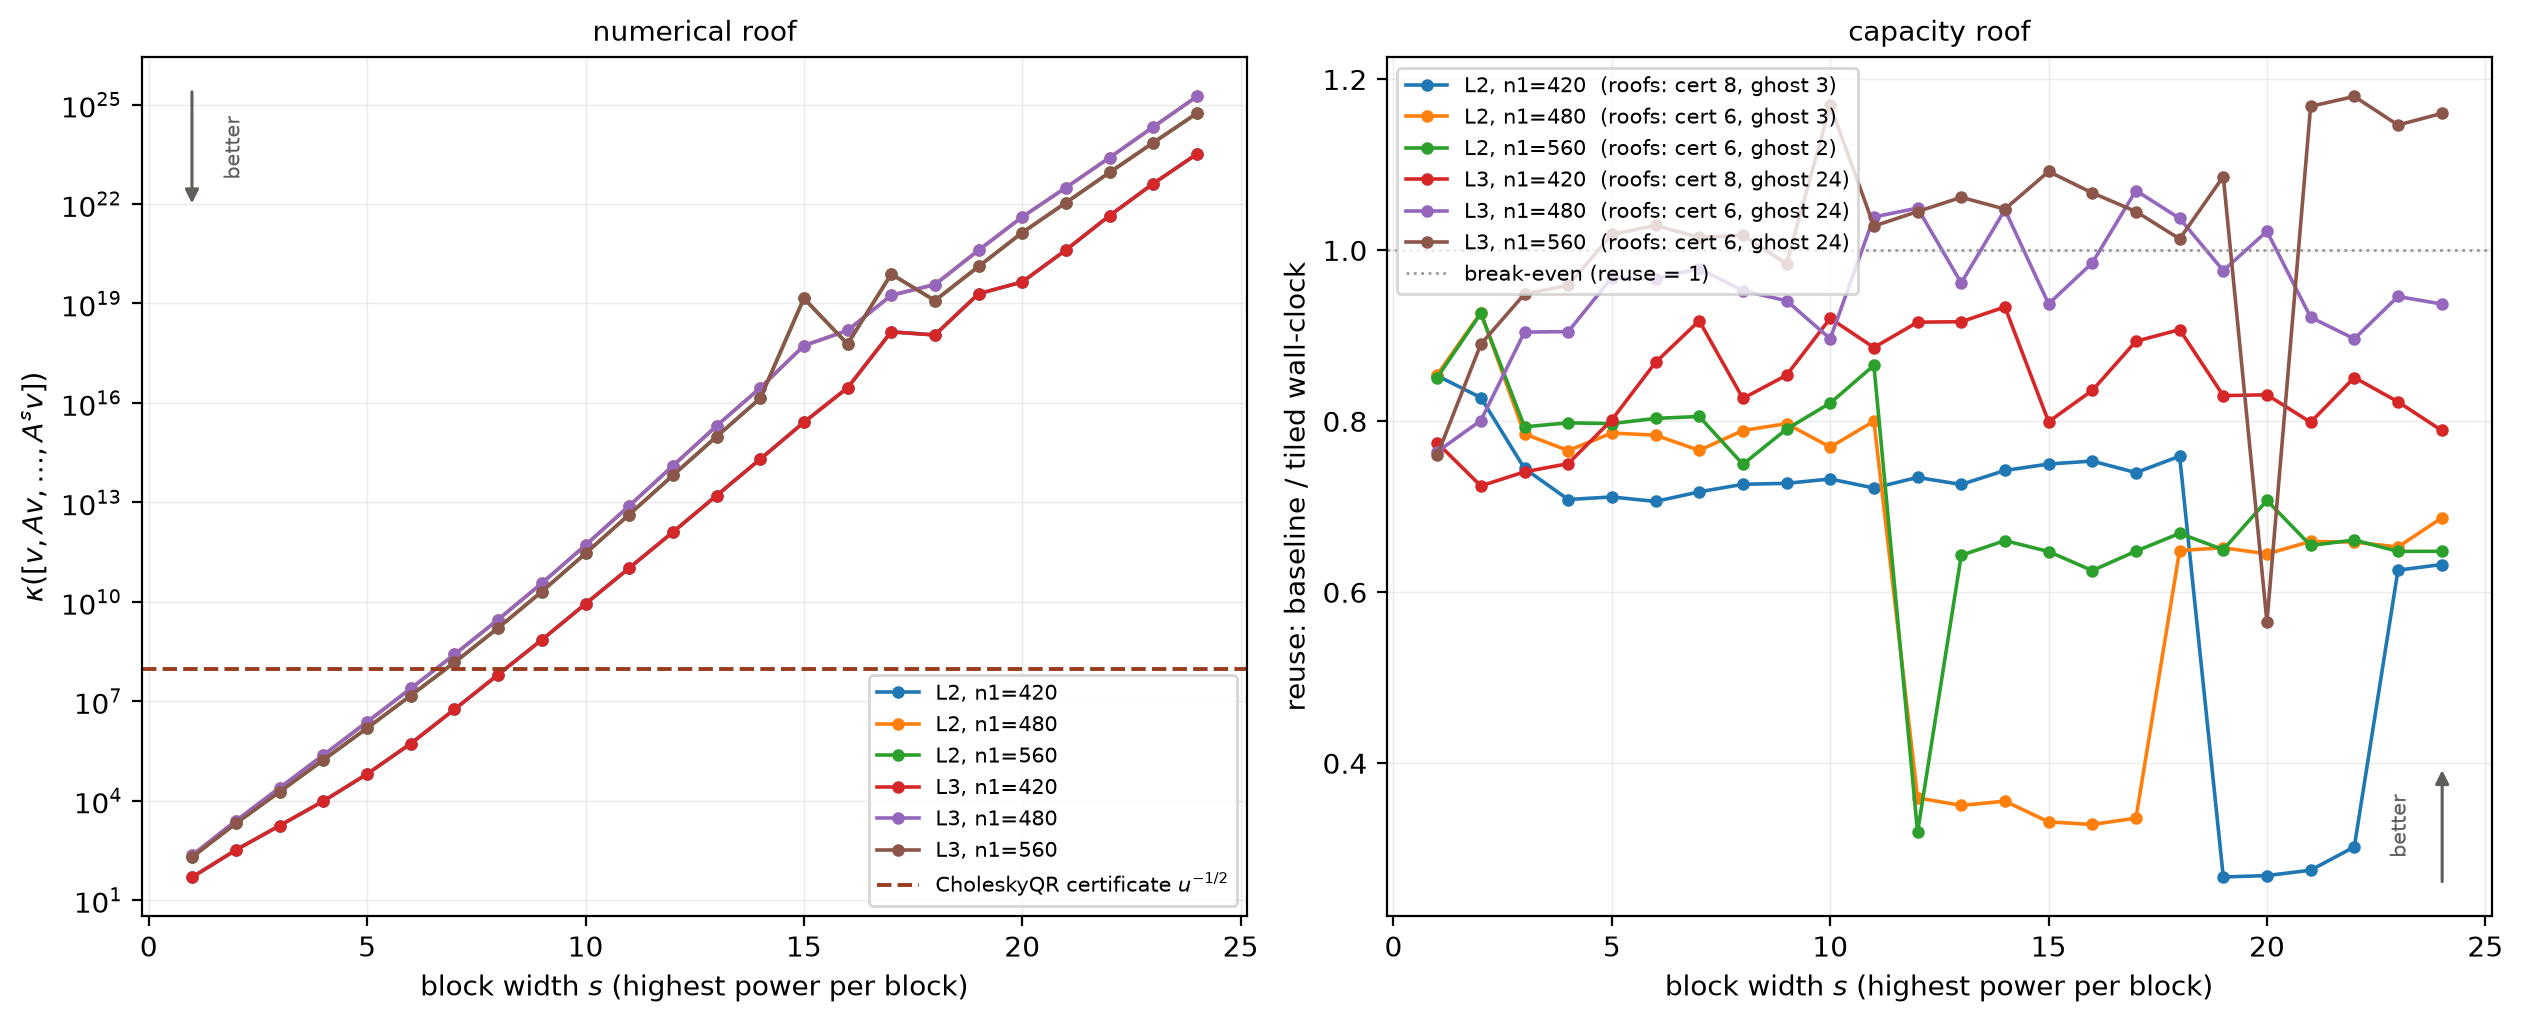
\includegraphics[width=0.95\textwidth]{regime_swidth.png}
\caption{The two roofs on the block width $s$: the numerical certificate and the ghost-zone
capacity, per tiling level.}
\label{fig:swidth}
\end{figure}

The distinction is actionable. Where the certificate binds, a better-conditioned basis
(Newton, Chebyshev \cite{hoemmen-2010,carson-2015}) converts the halo's slack into real
reductions. Where the ghost binds, only a thinner bandwidth or a coarser tiling level moves
it---a better basis buys nothing. Pinning $s$ assumes the first answer without measuring
it.

\subsection{The map, and where the real operator travels}\label{sec:map}

The measured real-operator points anchor the map; a predicted continuation carries the
operator to production grids. The continuation uses the \emph{same} a-priori placement the
instrument uses, and it is validated against the measured coordinates before it is trusted
to extrapolate---the replica reproduces every measured $(\Rv, \Rh)$ to better than
0.001\% (\Cref{tab:trajectory}, \Cref{fig:trajectory}).

\begin{table}[htbp]
\centering
\caption{The real operator's trajectory under grid refinement. Bisecting on $n$ puts the
$\theta_v$ crossing at $n \approx 73$.}
\label{tab:trajectory}
\begin{tabular}{@{}rrrrrl@{}}
\toprule
$n$ & $N$ & $m$ & $\Rv$ & $\Rh$ & \textbf{Source} \\
\midrule
10  & 1{,}000     & 6  & 0.0019         & 13.53  & measured \\
20  & 8{,}000     & 8  & 0.0175         & 1.87   & measured \\
25  & 15{,}625    & 8  & 0.036          & 0.904  & predicted \\
61  & 226{,}981   & 12 & 0.582          & 0.080  & predicted \\
74  & 405{,}224   & 13 & \textbf{1.063} & 0.047  & predicted (first above $\theta_v$) \\
120 & 1{,}728{,}000 & 15 & 4.74         & 0.0025 & predicted \\
\bottomrule
\end{tabular}
\end{table}

\begin{figure}[htbp]
\centering
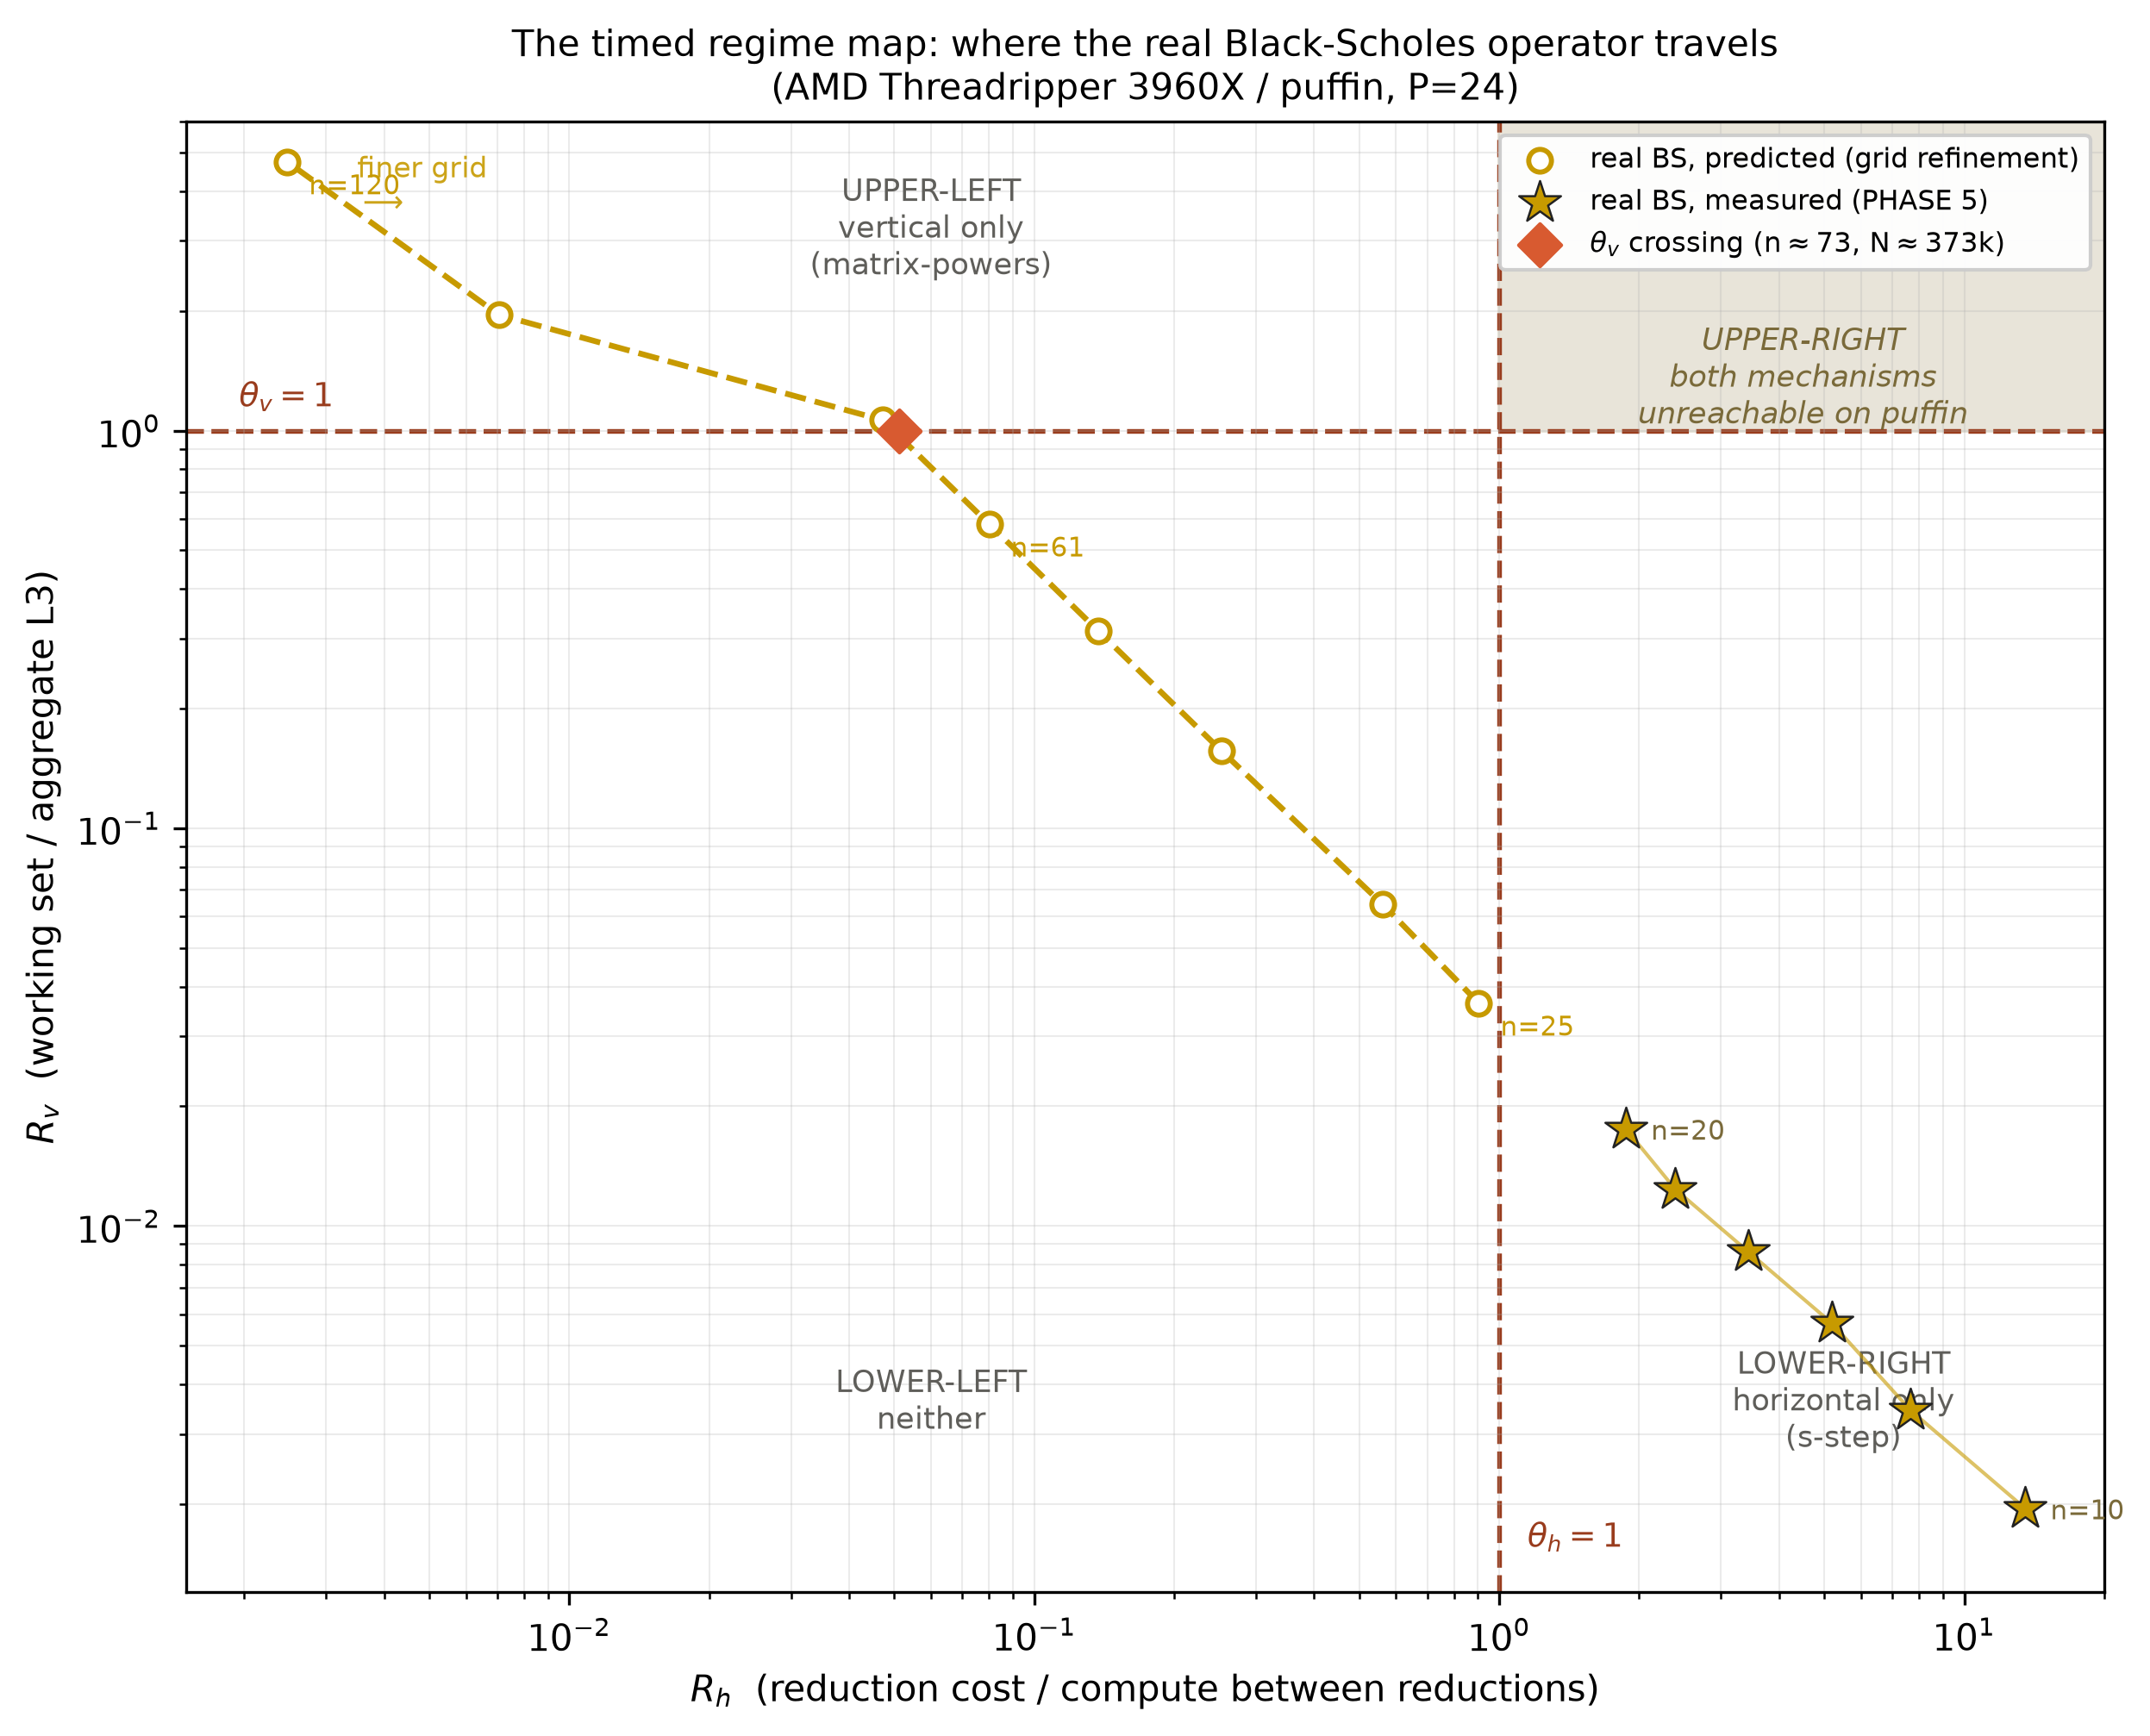
\includegraphics[width=0.95\textwidth]{regime_trajectory.png}
\caption{The regime map. The real Black--Scholes operator's refinement trajectory travels
lower-right $\to$ lower-left $\to$ upper-left, crossing $\theta_v$ just under $n = 74$ and
never entering the upper-right corner.}
\label{fig:trajectory}
\end{figure}

The interpretation of each leg:
\begin{itemize}
\item The measured points read $\Rh > 1$ only because the grids small enough to
  dense-eigensolve ($n \le 20$) sit far below any resolution a desk would price at. That is
  an irrelevant regime, not a grid where $s$-step pays.
\item At production resolution the operator is squarely in \textbf{vertical-only}
  territory. The mechanism the application needs is matrix-powers tiling; the mechanism the
  certificate work supports is $s$-step. They are not the same corner.
\item The upper-right corner is a \textbf{portability claim} on this hardware, not a
  measurement: reaching it needs an interconnect whose reduction cost is roughly
  25$\times$ puffin's, which means crossing a device or node boundary rather than a CCX
  boundary.
\end{itemize}

\subsection{Standing caveats}\label{sec:caveats}

Carried explicitly so no figure is read as claiming more than it measures.
\begin{itemize}
\item DRAM bytes are \textbf{modeled, not counted} (puffin's uncore counters need root);
  vertical-mechanism traffic claims are reconciled against the roofline, which is weaker
  evidence, and every such curve is labeled as a model.
\item $s_{\max}$ is reported at a \emph{chosen} tolerance of $\pm 1$ step, not a measured
  cross-platform noise floor; block \emph{counts} are quoted rather than raw $s_{\max}$.
  The cross-platform spread is one of the measurements the GPU study will supply
  (\Cref{sec:gpu}).
\item $\kappa(X)$ is dense-eigensolvable only to $N \le 32{,}768$: the certificate is
  validated well below where the performance claims live (real-operator control tops out at
  $N = 8{,}000$ against a production $N \approx 2.3 \times 10^5$). The structured
  computation lifts the cap for the synthetic operator only.
\item The upper-right corner is unreachable on a single-NUMA socket; its status is a
  portability argument, not a measurement.
\item Coordinates are \textbf{not portable across memory systems}: both axes must be
  re-derived from a new machine's constants before any port. A GPU's small L2, large
  bandwidth, and cheap on-chip reductions move both---which is exactly what
  \Cref{sec:gpu} sets out to exploit.
\end{itemize}

%%%%%%%%%%%%%%%%%%%%%%%%%%%%%%%%%%%%%%%%%%%%%%%%%%%%%%%%%%%%%%%%%%%%%%%%%%%%%%%%%%%
\section{Toward GPUs: falsifying the map}\label{sec:gpu}

\emph{This section describes work in progress: the design is fixed and the first
instruments exist, but no GPU crossover has yet been measured. It is included because the
design is itself a result of the CPU study.}

\subsection{The falsification test}

The CPU study's central claim is that $\Rv$ and $\Rh$ are \emph{dimensionless}---ratios,
not times---so a reader can place their own operator and machine on the map. That claim
has never been tested against a machine whose memory system differs in kind: puffin is one
socket, one NUMA node, one cache hierarchy. The GPU work is therefore not a port. It is
the falsification test of the map's central claim, and both outcomes are informative:
either the coordinates, recomputed from GPU constants, predict the measured GPU crossover
at $\theta_v = \theta_h = 1$ and the dimensionless framing is vindicated; or they do not,
the map is scoped to CPU-like memory systems, and \emph{why} it fails names the missing
term. The deliverable is a placed and \emph{verified} crossover, not a running GPU kernel.

Two available GPUs make a near-controlled pair, and the pair is a better instrument than
either card alone (\Cref{tab:gpus}): the memory systems are nearly identical---same 6\,MB
L2, same bandwidth class---while the FP64 rate differs by ${\sim}12\times$. The two cards
hold the map's vertical axis roughly fixed and vary only the compute roof.

\begin{table}[htbp]
\centering
\caption{The two-GPU controlled pair.}
\label{tab:gpus}
\begin{tabular}{@{}lcccc@{}}
\toprule
 & \textbf{L2} & \textbf{Memory BW} & \textbf{FP64 peak} & \textbf{FP64:FP32} \\
\midrule
RTX 3090 (consumer, puffin)      & 6\,MB & ${\sim}936$\,GB/s & ${\sim}0.56$\,TFLOP/s & 1/64 \\
Tesla V100 (datacenter, cluster) & 6\,MB & ${\sim}900$\,GB/s & ${\sim}7.0$\,TFLOP/s  & 1/2  \\
\bottomrule
\end{tabular}
\end{table}

That lever tests the map's hidden precondition. Both axes are \emph{communication} axes,
presupposing the kernel is on the memory side of the roofline; a hard-throttled FP64 rate
does not move a point around the map, it throws the point \emph{off} the map into
compute-bound territory the map does not chart. Placement is therefore gated by an explicit
roofline check---is $AI \cdot BW_{\text{achieved}} < \text{FLOP/s}_{\text{peak}}$ in the
relevant precision?---evaluated before the map is read. The gate is itself a prediction the
pair measures: \textbf{pass on the V100} (FP64 memory-bound), \textbf{fail on the 3090}
(FP64 compute-bound). A map that predicts where it itself stops applying is a stronger
vindication of the dimensionless framing than any single-machine crossover; the 3090 is
the designed negative arm of the experiment, not a hazard to route around.

\subsection{What transfers, and what breaks}

Everything machine-independent transfers unchanged: the synthetic operator, the tensor law
\eqref{eq:tensor-law}, the numerics gates C1--C6, the reduction ledger, the CholeskyQR2
certificate, and the thresholds $\theta_v = \theta_h = 1$ themselves---a ratio crosses 1
where supply meets demand, which is what makes the thresholds portable. Only the
coordinates are recomputed. Three things break structurally, not by constant swap:

\begin{itemize}
\item \textbf{The denominator of $\Rv$.} On the CPU each engaged CCX brings its own L3
  slice, so aggregate last-level cache scales with the team. A GPU's L2 is a single fixed
  block shared by every streaming multiprocessor: engaging more of the device adds zero
  cache, so within one device $\Rv$ stops being a function of the team size at all. This is
  the event that \emph{decouples the two axes}. On the CPU both coordinates shared the
  parallelism knob ($\Rv \sim 1/P$, $\Rh \sim P\log P$), which is why
  $\Rv \cdot \Rh$ collapsed to a $P$-independent constant (${\sim}0.04$ on puffin)---the
  invariant that made the upper-right corner unreachable on one node. If the decoupling
  holds, that cancellation is broken and the corner may open for structural reasons rather
  than because of a slow interconnect; whether it does is the highest-impact open question,
  and it is being resolved on paper before any kernel is written.
\item \textbf{The numerator of $\Rh$.} The CPU model has two reduction tiers and one
  saturation constant \eqref{eq:treduce}. A GPU reduction crosses at least five
  qualitatively different tiers (\Cref{tab:tiers}), and the grid tier carries kernel-launch
  latency, which has no CPU analogue---a fixed cost per reduction independent of tree
  depth. Two parameters cannot express five tiers: the machine model needs a tier vector,
  and the reduction-cost predictor needs to walk it. The ladder is the instrument, not an
  obstacle: three reachable rungs with distinct costs (on-device, intra-node across PCIe,
  inter-node across the fabric) place the \emph{same} problem at three different $\Rh$
  values, so holding the problem and device fixed while changing only the reduction
  hardware traverses the horizontal axis directly, converting $\theta_h$ from a shaded
  prediction into a measured crossing.
\item \textbf{The reuse model.} The CPU scatter knob costs a factor of a few in cache-line
  reuse; on a GPU the same permutation defeats warp coalescing and can serialize a
  32-thread gather into 32 transactions. The scatter axis becomes \emph{more}
  discriminating, but the reuse model must be recalibrated from scratch.
\end{itemize}

\begin{table}[htbp]
\centering
\caption{The reduction-tier ladder on the target cluster (two nodes, one Tesla V100 per
node, PCIe interconnect without NVLink). Every tier cost must be measured, never assumed.}
\label{tab:tiers}
\begin{tabular}{@{}lp{5.2cm}lp{3.4cm}@{}}
\toprule
\textbf{Tier} & \textbf{Mechanism} & \textbf{Scope} & \textbf{Cost class} \\
\midrule
Warp   & register shuffle                & on-die     & near-free, no memory traffic \\
Block  & shared memory + barrier         & on-die     & cheap, on-chip \\
Grid   & atomics or a second launch      & on-die     & expensive; carries launch latency \\
Device & PCIe + cross-socket link        & intra-node & expensive; a genuine cross-socket hop \\
Node   & network fabric                  & inter-node & dominant; fabric identity to confirm \\
\bottomrule
\end{tabular}
\end{table}

\subsection{Phasing}

The study preserves predict-then-measure throughout: coordinates are predicted a priori
from recomputed constants and never fitted to the measurement. Phase 0 (paper, no code)
resolves whether the $\Rv \cdot \Rh$ invariant survives the chosen definition of team
size, and whether an upper-right window even exists under the 16\,GB device-memory ceiling
at a resolution the pricing problem would actually use. Phase 1 builds the calibration
instruments---a per-tier reduction calibration, a GPU STREAM for the achieved bandwidth
roof, and an interconnect probe. Phase A lands the single-GPU vertical crossover and
evaluates the roofline gate on both cards (predicted: V100 on-map, 3090 off-map); it also
supplies the cross-platform $s_{\max}$ spread that \Cref{sec:caveats} lists as missing,
since a GPU is a maximally different floating-point platform. Phase B traverses the
reduction ladder for the horizontal crossover and the upper-right corner---the corner
puffin could not reach, either reached-and-measured or shown empty with a mechanism.
Phase C places the real Black--Scholes operator at production resolution on the V100 map
and delivers the two-GPU falsification verdict.

\subsection{Open questions and risks}

Four items are recorded here because each would change the design, and each is a finding
either way it resolves. First, the $\Rv \cdot \Rh$ invariant question above: if the
decoupling holds, the upper-right corner opens structurally; if a sensible definition of
team size re-couples the axes, the corner stays governed by the same invariant with a new
constant. Second, whether an upper-right window exists at all under the 16\,GB
device-memory ceiling at usable resolution: on the CPU, a corner that ``opened'' turned
out to be a 1\%-wide artifact of freezing one axis while sliding the other, so the three
constraints (spill the 6\,MB L2 with margin, keep the reduction dominant, fit in 16\,GB)
must be solved jointly before a run is aimed at the intersection. If the window is empty,
the honest claim is a \emph{measured} boundary rather than a \emph{reached} corner. Third,
kernel-launch latency: if it dominates every grid-level reduction, the tier model
collapses to a constant and the horizontal mechanism becomes uninteresting---itself a
result, but a different one. Fourth, occupancy: shared-memory tiling trades against it,
and if that tradeoff proves independent of both coordinates, the map does not extend to
GPUs without a third dimension---which would be stated, not hidden by fixing occupancy at
one value.

%%%%%%%%%%%%%%%%%%%%%%%%%%%%%%%%%%%%%%%%%%%%%%%%%%%%%%%%%%%%%%%%%%%%%%%%%%%%%%%%%%%
\section{Conclusion}\label{sec:conclusion}

This thesis set out to decide when communication-avoiding reformulations of a Krylov
exponential integrator pay for a multi-asset option-pricing problem, and to make the
answer portable. The instrument for that answer is a dimensionless regime map whose
coordinates are predictors---computed from the problem, the spectrum, and machine
constants before any run---and whose boundaries are tested by measurement.

On the numerical side, the certified $s$-step block width is predicted from the spectrum
alone and verified integer-exact on 20 of 21 runs; a confound control shows safety is a
property of the spectrum, not of the Krylov dimension; a log-robustness law bounds the
damage non-normality does to the prediction (slope 0.069 in decades per decade of
eigenvector conditioning for the constant-coefficient family, $4\times$ steeper for
variable coefficients, the real operator under one $s$-step everywhere); and a closed-form
tensor law gives the geometric growth of $\kappa(X)$ with asset dimension, along with the
warning that the dense eigensolver value is meaningless once the spectrum degenerates.

On the measurement side, the study delivers three placed results. The horizontal
mechanism is a null result with a mechanism: an 11--16$\times$ cut in reduction count
moves wall-clock by nothing, because the reduction primitive was never the bottleneck and
Gram--Schmidt is bandwidth-bound---exactly as the map's $\Rh = 0.080$ predicted. The
vertical mechanism is a shortfall with a mechanism: cache-blocked matrix powers loses to
its own halo arithmetic at L2 tile sizes and to a residency-insensitive cap at L3, so the
predicted crossover $\theta_v$ remains untested by this kernel rather than refuted. And
the real operator's trajectory under refinement---lower-right, lower-left, upper-left,
crossing $\theta_v$ near $n = 74$---says the mechanism the application needs at production
resolution is matrix-powers tiling, not $s$-step, and that the upper-right corner is
structurally unreachable on a single-NUMA socket.

\subsection{Future work}

Three lines of work follow directly from the measured boundaries, beyond the GPU study
already outlined.

\emph{A better-conditioned basis where the certificate binds.} The block-width analysis
(\Cref{sec:swidth}) shows the numerical roof binding at L3 tile sizes while the ghost roof
still has slack. There, and only there, replacing the monomial basis with a Newton or
Chebyshev basis \cite{hoemmen-2010,carson-2015} converts that slack into real reductions;
where the ghost binds, a better basis buys nothing. The map now says where each investment
pays.

\emph{Counted, not modeled, DRAM traffic.} The vertical-mechanism evidence is reconciled
against the roofline because puffin's uncore counters require root access. Repeating the
sweep on a machine with accessible memory controllers would upgrade the traffic claims
from model to measurement---and either close or widen the gap between the 4--8$\times$
modeled ceiling and the measured shortfall.

\emph{A structural result for the real-operator certificate gap.} The tensor identity
closes the computability gap for the synthetic operator because that operator is a pure
Kronecker sum; the real Black--Scholes operator with all-pairs correlation is not. Brute
force does not help---at production resolution the eigenvector matrix alone would need
hundreds of gigabytes---so what is needed is a decomposition of the correlated operator as
a Kronecker backbone plus a correlation perturbation, bounding its $\kappa(X)$ as a
perturbation of the factorizable part. That is an analysis problem, not a bigger
eigensolve.

The map's central claim---that its coordinates transfer---remains its least-tested one,
and the GPU study of \Cref{sec:gpu} is designed to falsify it on a memory system that
differs in kind, with a controlled two-GPU pair whose roofline gate the map must predict.
That work is in progress; the map now exists to tell it what to build.

\newpage
\addcontentsline{toc}{section}{References}
\bibliographystyle{plainurl}
\bibliography{Bibliography.bib}

\end{document}
